\documentclass{ws-ijbc}

%%%%%%%%%%%%%%%%
% Instructions %
%%%%%%%%%%%%%%%%
% Set the document class and settings to match the final document that these figures_raw will be included into
% This will output a pdf with a page for each figure, nicely cropped according to picture dimenstions as defined below in the `Figure' Section. Inlcude in the final document by using package 'graphicx' and command \includegraphics[page=<page of figure>]{figures_raw.pdf}
% The following package is used to create the cropping mentioned above, and apparently should be the last loaded package: \usepackage[active,tightpage]{preview}
% The following command re-writes the figure enviroment to become a preview enviroment - without this spacing is off, and captions and labels may appear
%\renewenvironment{figure}[1][]{%
%	\begin{preview}%
%		\renewcommand{\caption}[2][]{}}
%	{\end{preview}}

%%%%%%%%%%%%%%%%%
% Load Packages %
%%%%%%%%%%%%%%%%%
\usepackage{epsfig}
\usepackage{amssymb}
\pagestyle{empty}
\usepackage{epstopdf}
\usepackage{mathrsfs}
\usepackage{amsmath}
\usepackage{graphicx}
\usepackage{array}
\usepackage{xcolor}    % \nopagecolor
\usepackage{fp}
\usepackage[T1]{fontenc}
\usepackage{bm}    % boldmath \bm{}
\usepackage[pdftex,active,tightpage]{preview}    % should be loaded lasts
% adjust borders added to figures_raw: left, lower, right and upper borders. - useful to increase lower border not to cut off labels placed below figure bounds. 
\renewcommand{\PreviewBbAdjust}{0mm -0.25mm 0mm 0mm}
\renewenvironment{figure}[1][]{%
	\begin{preview}%
		\renewcommand{\caption}[2][]{}}
	{\end{preview}}

\setlength{\unitlength}{1mm}

%%%%%%%%%%%%%%%%%%%%%%%%%%%%%%%%%%%%%%%%%%%%%%%%
% Get various dimensions for the documentclass %
%%%%%%%%%%%%%%%%%%%%%%%%%%%%%%%%%%%%%%%%%%%%%%%%
\makeatletter
\newcommand*{\getlength}[1]{\strip@pt\dimexpr0.035136\dimexpr#1\relax\relax}
\newcommand{\showfont}{%
encoding: \f@encoding{},\\
family: \f@family{},\\
series: \f@series{},\\
shape: \f@shape{},\\
size: \f@size{} pt,\\
text height: \getlength{\the\textheight} cm,\\
text width:     \getlength{\the\textwidth} cm}
\makeatother









\begin{document}








%\begin{figure}
%	\begin{picture}(20,5)(0,0)
%		\showfont
%	\end{picture}
%\end{figure}
%\newpage


%%%%%%%%%%%%%%%%
%%% Figure 1: Critical manifold %%%
%%%%%%%%%%%%%%%%
\nopagecolor
\begin{figure}
	\begin{picture}(85,44)(5.5,6.5)
	\put(10.25,10){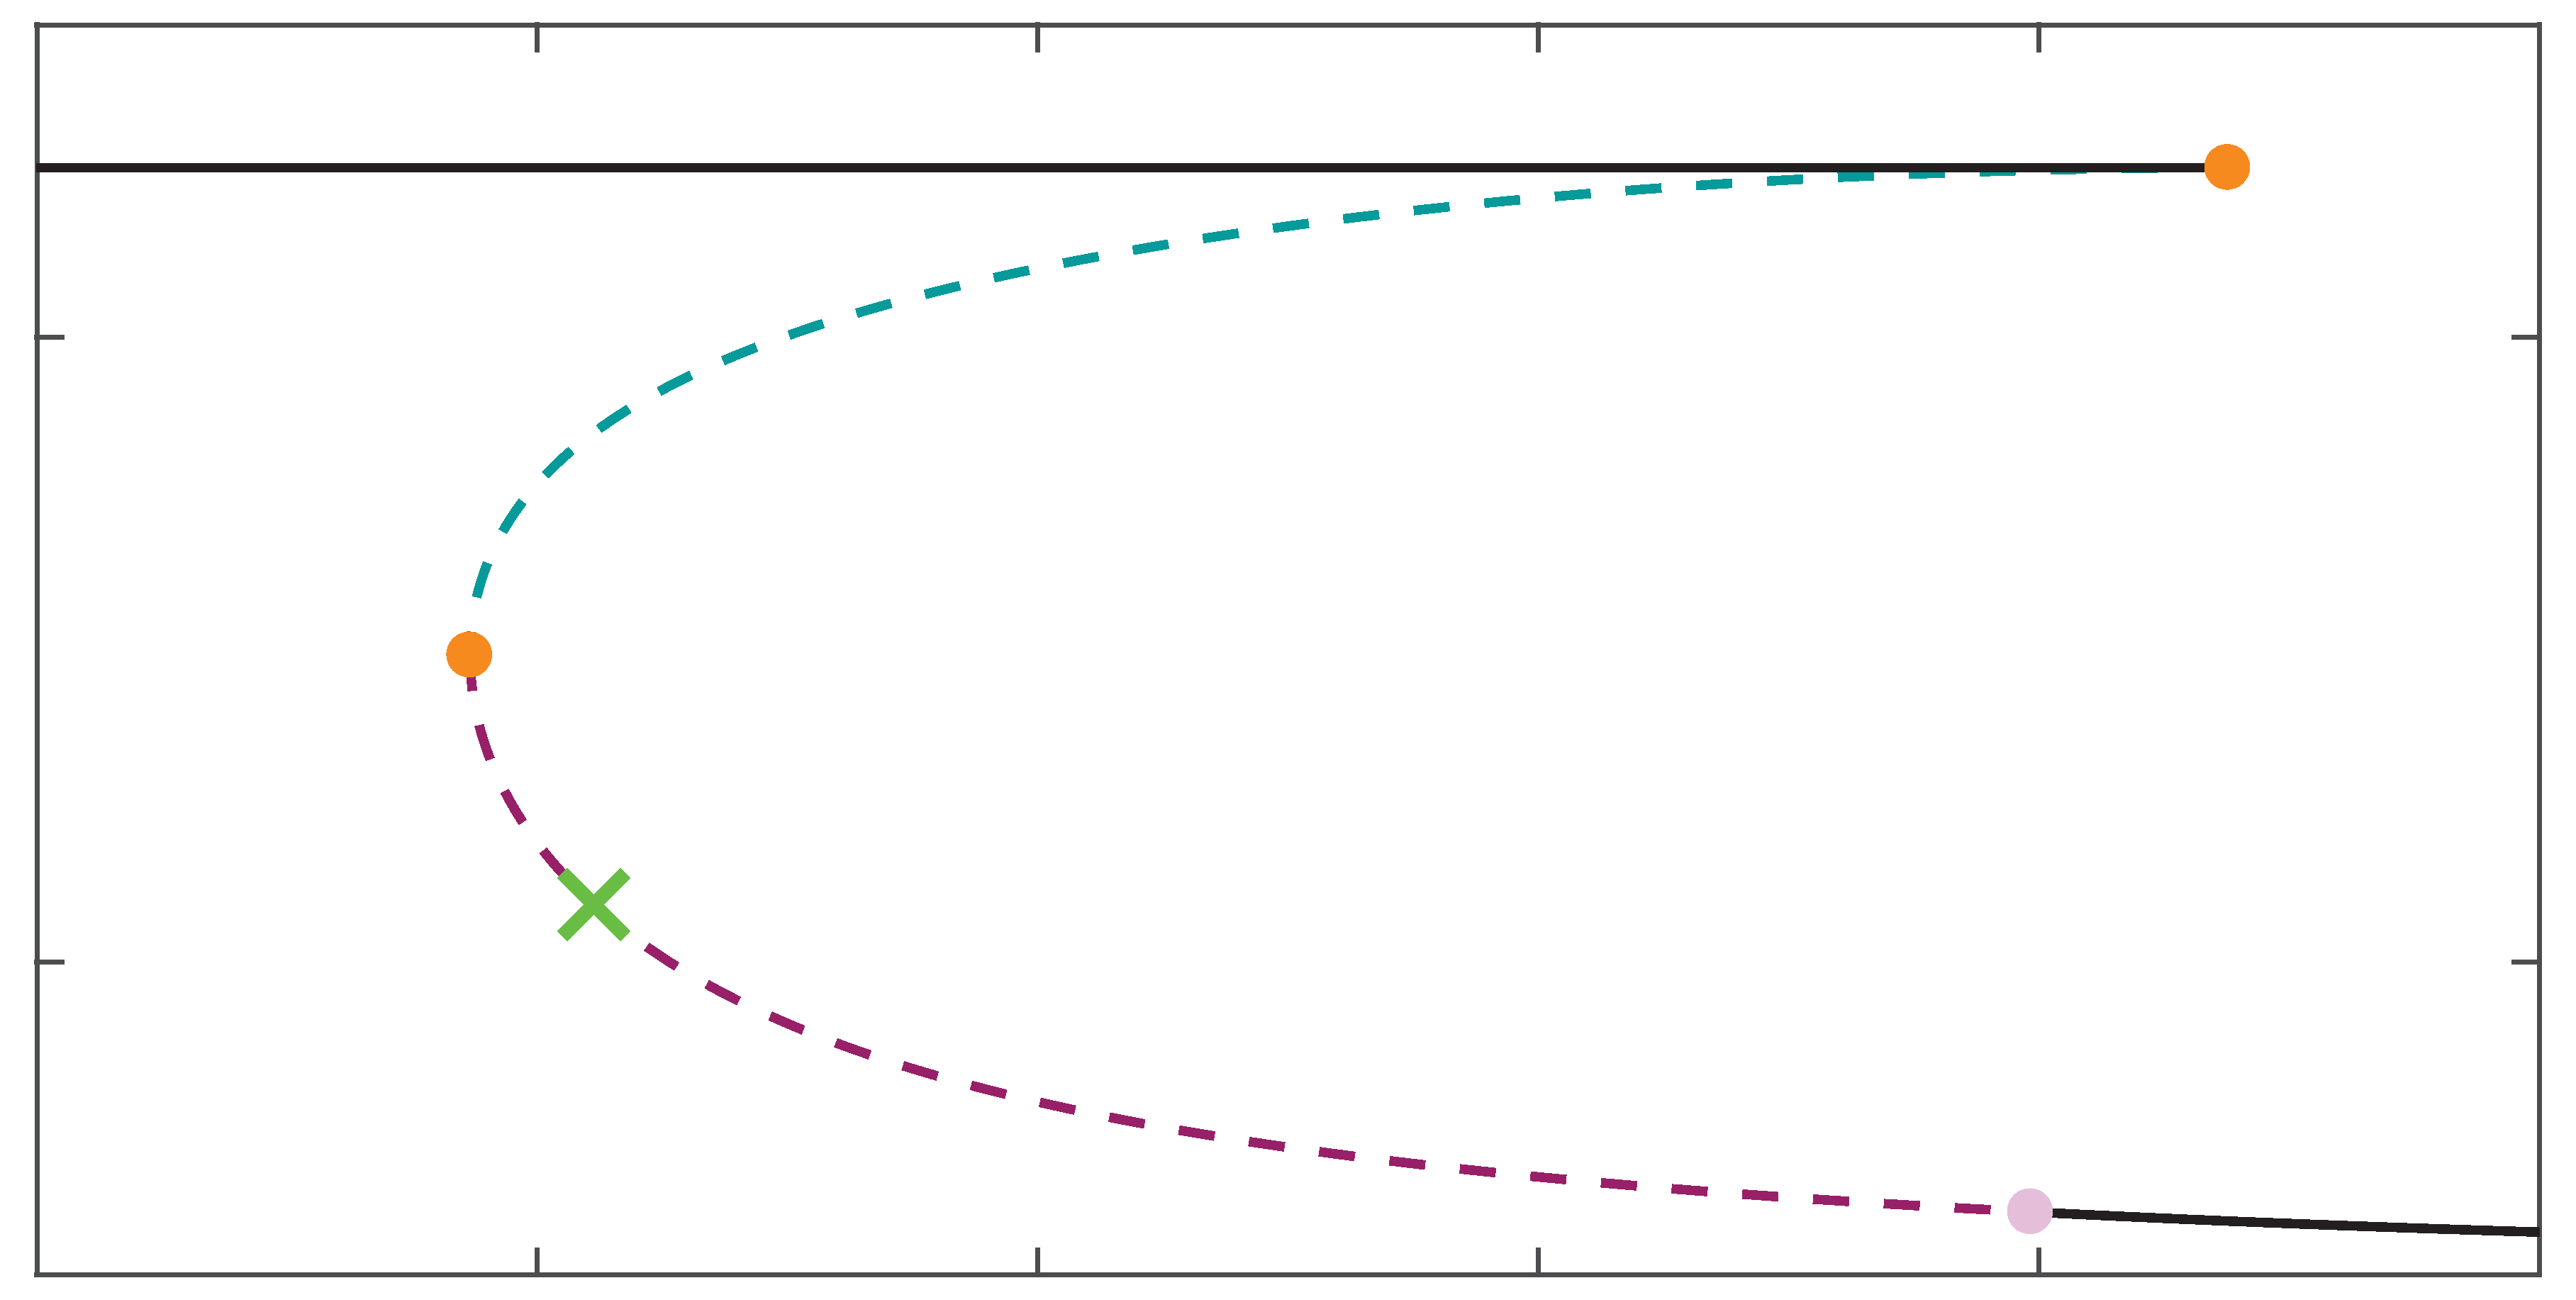
\includegraphics[width=8cm]{./figures_raw/paper_critical.eps}}
	\put(81,44){$F_1$}
        \put(19,29){$F_2$}
        \put(72.5,13.5){$H$}
        \put(80,13){$C^4_-$}
        \put(20,41.5){$C^4_+$}
        \put(50,40){$C^3$}
        \put(50,15){$C^2$}
        \put(7,46){$A$}
        \put(6,39){\footnotesize $9.0$}
        \put(6,19){\footnotesize $3.0$}
	\put(24.5,7.5){\footnotesize $0.3$}
	\put(40.4,7.5){\footnotesize $0.5$}
	\put(56.4,7.5){\footnotesize $0.7$}
	\put(72.2,7.5){\footnotesize $0.9$}
	\put(86,6.9){$B$}
	\put(25,20){$q$}
	\end{picture}
	\caption{}
\end{figure}
\newpage

%%%%%%%%%%%%%%%%%%
%%%% Figure 2: Tube figure %%%
%%%%%%%%%%%%%%%%%%

\begin{figure}
	\begin{picture}(114.75,63)(94.75,97)
	    \put(100,100){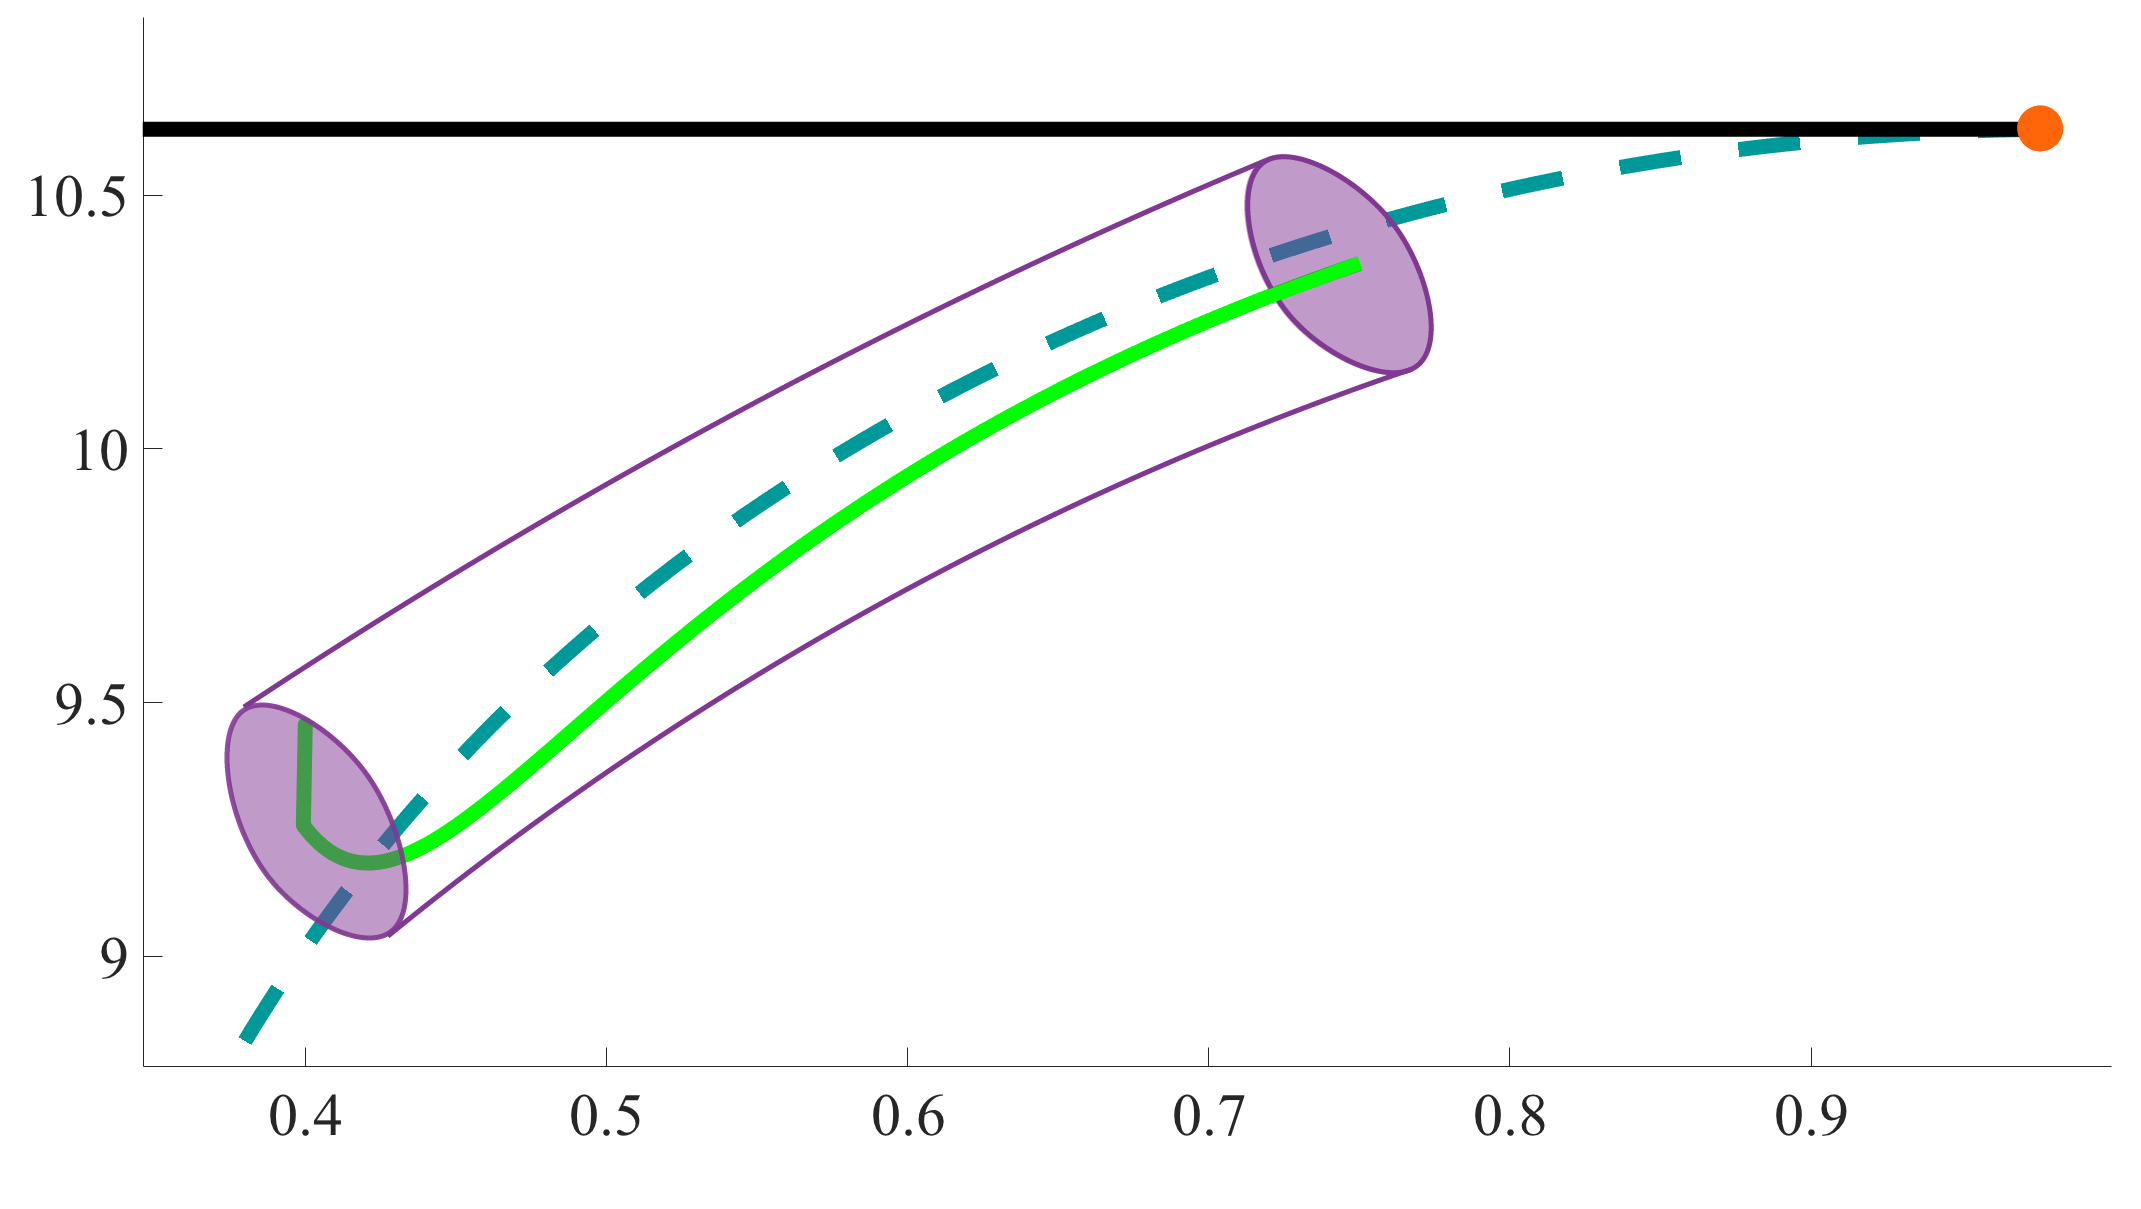
\includegraphics[width=11cm]{./figures_raw/paper_slow.eps}}
	    \put(196.5,153.5){$F_1$}
	    \put(173.5,148){$D^s_\delta(B_{\mathrm{out}})$}
	    \put(107,127){$D^s_\delta(B_{\mathrm{in}})$}
	    \put(121.5,110){$C^3$}
	    \put(120,151){$C^4_+$}
	    \put(147.5,133.5){$S^3$}
	    \put(148,138.25){$\big\uparrow$}
	    \put(97.5,156){$A$}
	    \put(95,143.5){\footnotesize $9.75$}
	    \put(95,114.25){\footnotesize $7.25$}
            \put(206,97){$B$}
            \put(120.75,98){\footnotesize$0.3$}
            \put(142.25,98){\footnotesize$0.5$}
            \put(163.8,98){\footnotesize$0.7$}
            \put(185.25,98){\footnotesize$0.9$}
	\end{picture}
	\caption{}
\end{figure}

\newpage


%%%%%%%%%%%%%%%%%%%%%%%%%%%%
%%% Figure 3: Stable manifold numerical set up %%%
%%%%%%%%%%%%%%%%%%%%%%%%%%%%

\begin{figure}
\begin{picture}(172.75,89)(2,-0.5)
\put(0,45){
	\begin{picture}(85,43)(5,7)
	\put(10.25,10){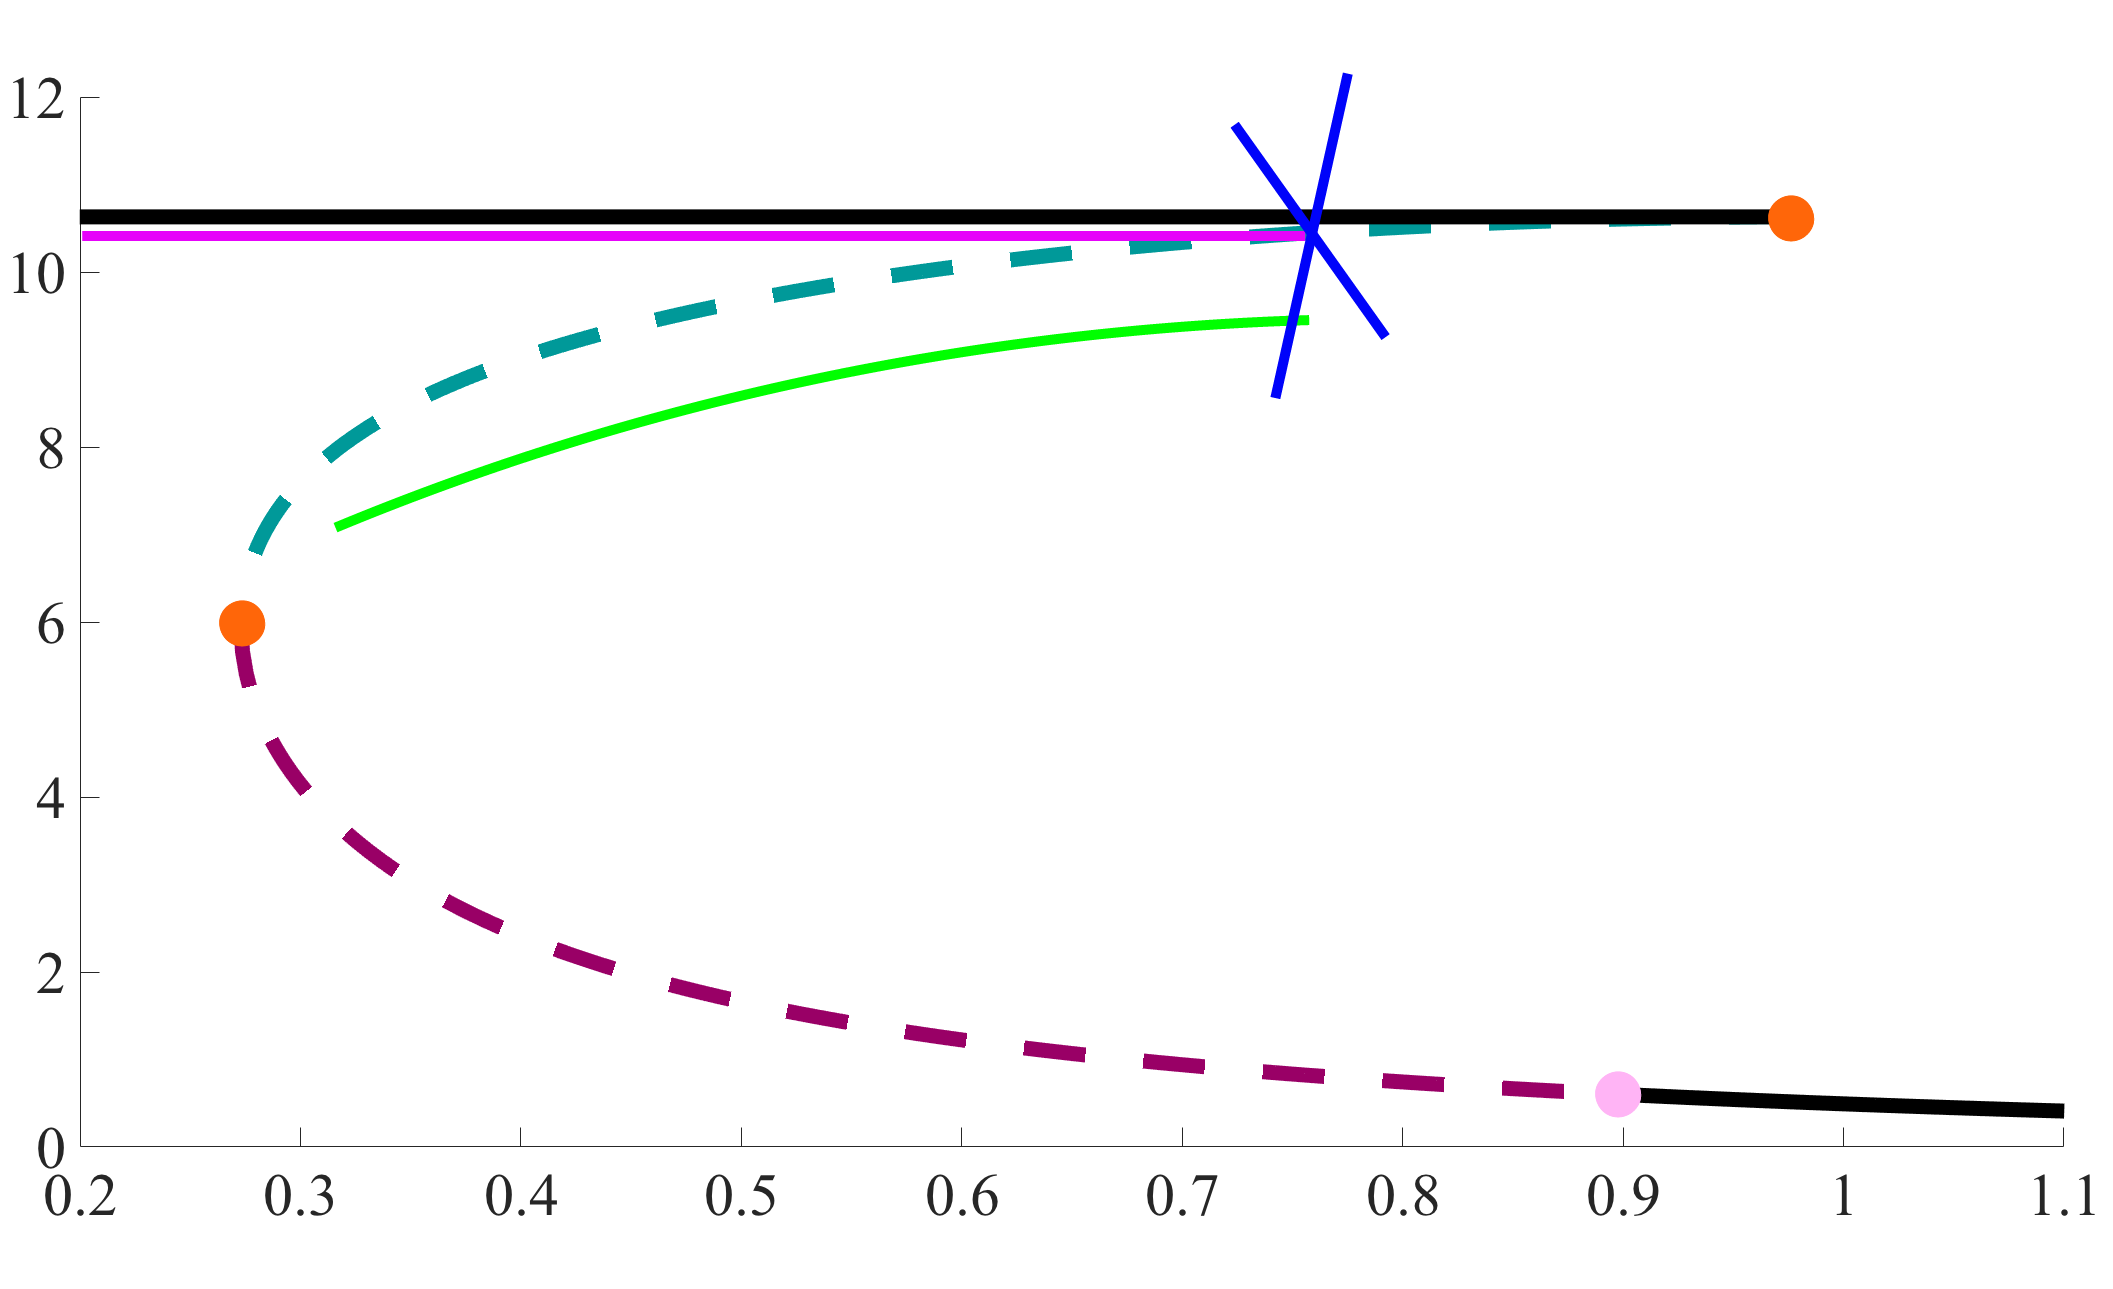
\includegraphics[width=8cm]{./figures_raw/step1.eps}}
        \put(72,37.75){$E^s(p_{\mathrm{out}})$}
        \put(20,41){$\Sigma_0$}
        \put(50,46.5){$C^4_+$}
	\put(81,44){$F_1$}
        \put(19,29){$F_2$}
        \put(72.5,13.5){$H$}
        \put(80,13){$C^4_-$}
        \put(50,38){$S^3$}
        \put(50,15){$C^2$}
        \put(7,46){$A$}
        \put(6,39){\footnotesize $9.0$}
        \put(6,19){\footnotesize $3.0$}
	\put(24.5,7.5){\footnotesize $0.3$}
	\put(40.4,7.5){\footnotesize $0.5$}
	\put(56.4,7.5){\footnotesize $0.7$}
	\put(72.2,7.5){\footnotesize $0.9$}
	\put(86,6.9){$B$}
	\put(13,13.5){(a)}
	\put(25,20){$q$}
	\end{picture}
	\caption{}
	}

\put(88,45){
	\begin{picture}(85,43)(5,7)
	\put(10.25,10){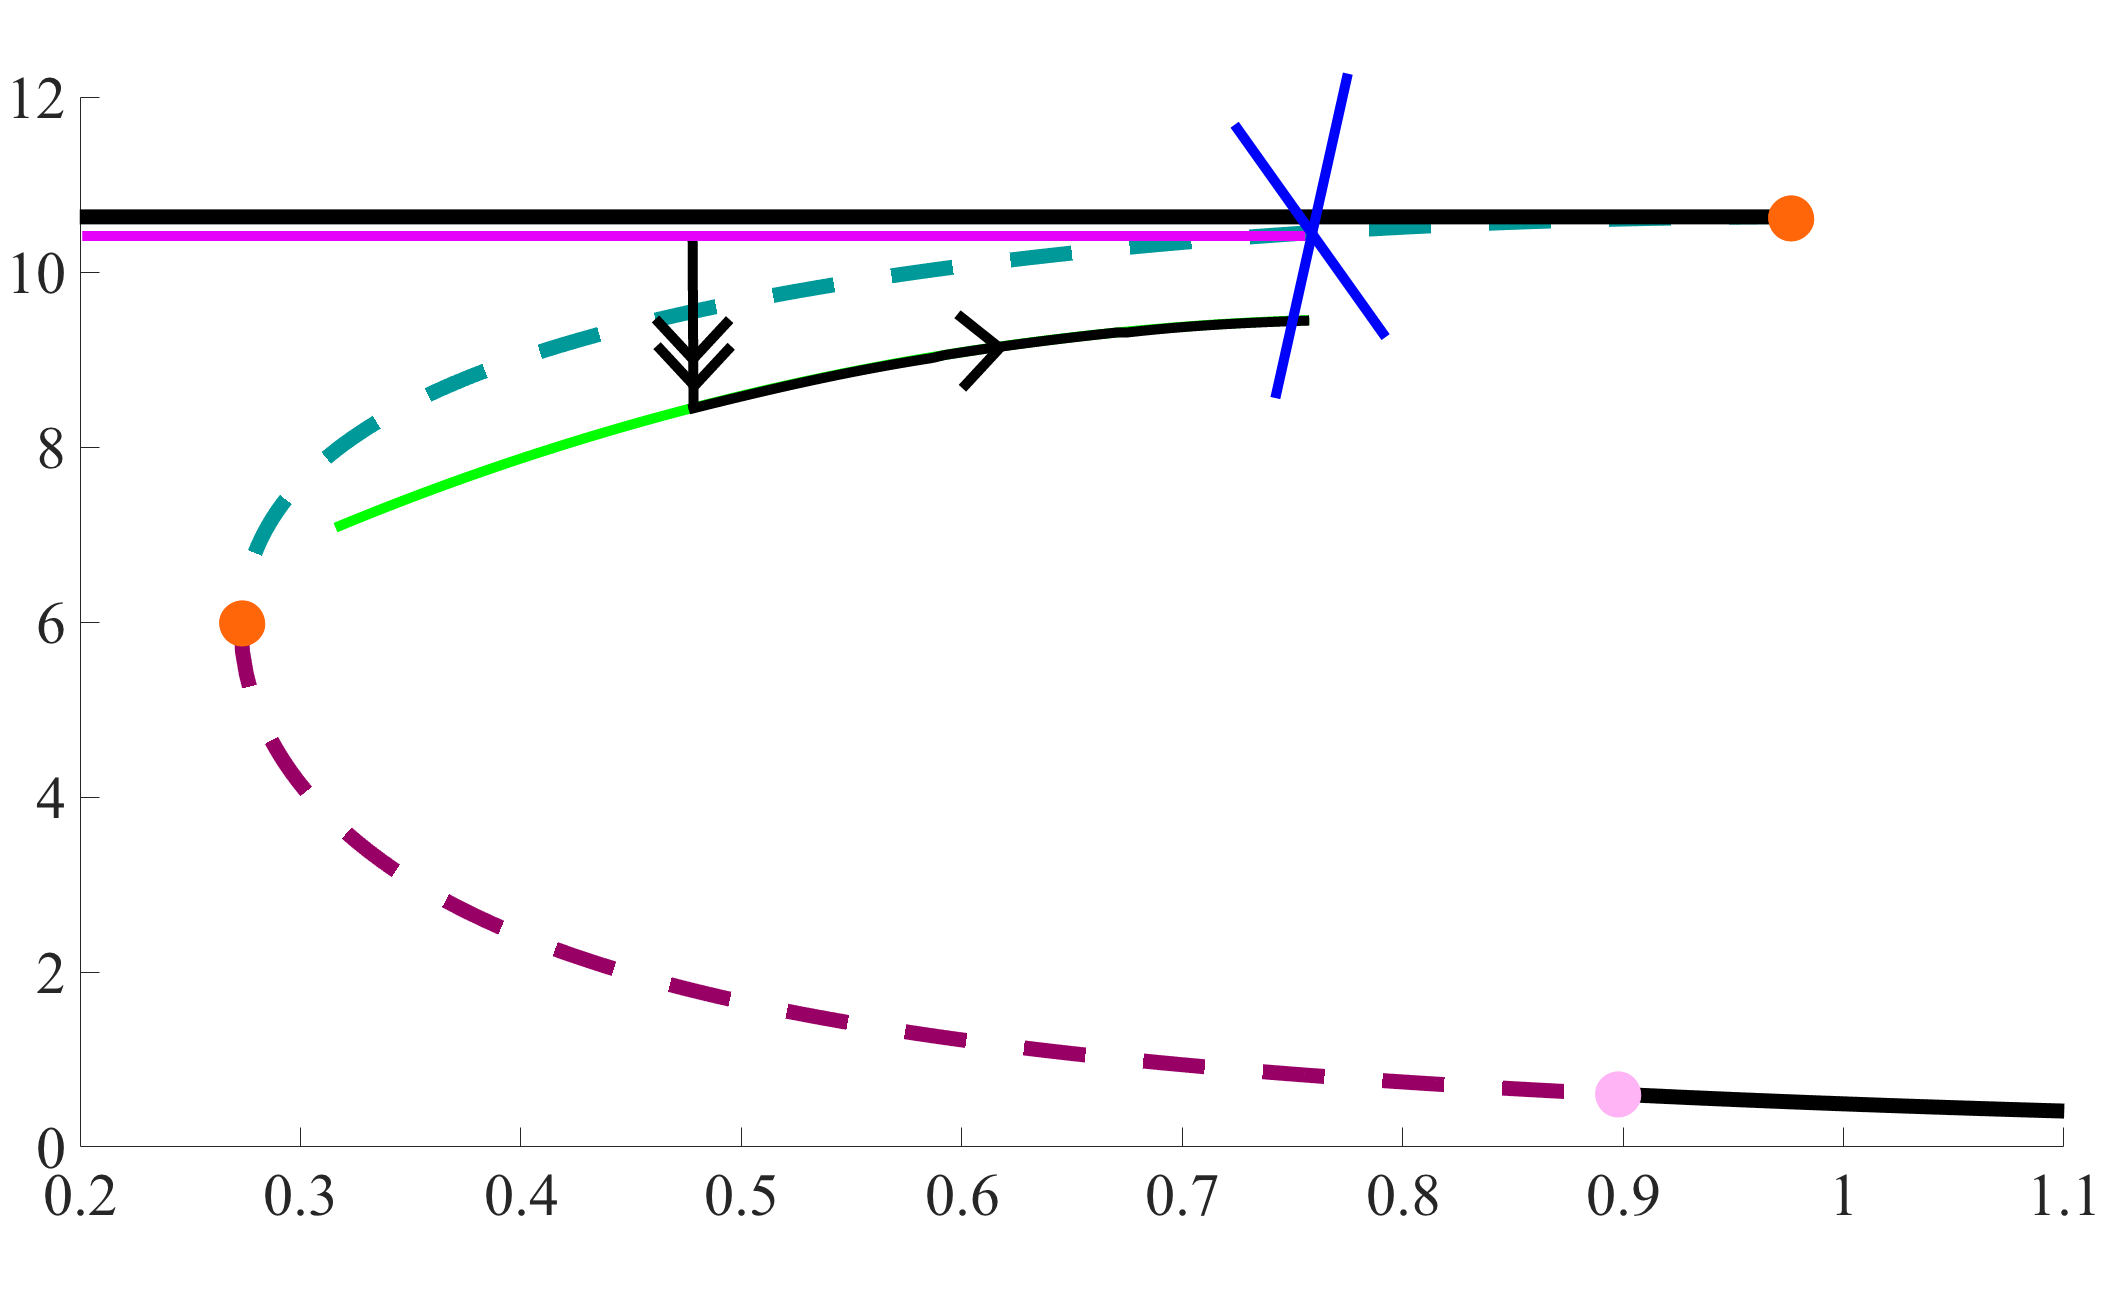
\includegraphics[width=8cm]{./figures_raw/step2.eps}}
        \put(72,37.75){$E^s(p_{\mathrm{out}})$}
        \put(20,41){$\Sigma_0$}
        \put(50,46.5){$C^4_+$}
	\put(81,44){$F_1$}
        \put(19,29){$F_2$}
        \put(72.5,13.5){$H$}
        \put(80,13){$C^4_-$}
        \put(7,46){$A$}
        \put(50,15){$C^2$}
         \put(37,46.5){$\mathbf{u}(0)$}
        \put(55,39.25){$\mathbf{u}$}
        \put(6,39){\footnotesize $9.0$}
        \put(6,19){\footnotesize $3.0$}
	\put(24.5,7.5){\footnotesize $0.3$}
	\put(40.4,7.5){\footnotesize $0.5$}
	\put(56.4,7.5){\footnotesize $0.7$}
	\put(72.2,7.5){\footnotesize $0.9$}
	\put(86,6.9){$B$}
	\put(13,13.5){(b)}
	\put(25,20){$q$}
	\end{picture}
	\caption{}
	}
	
\put(0,0){
	\begin{picture}(85,43)(5,7)
	\put(10.25,10){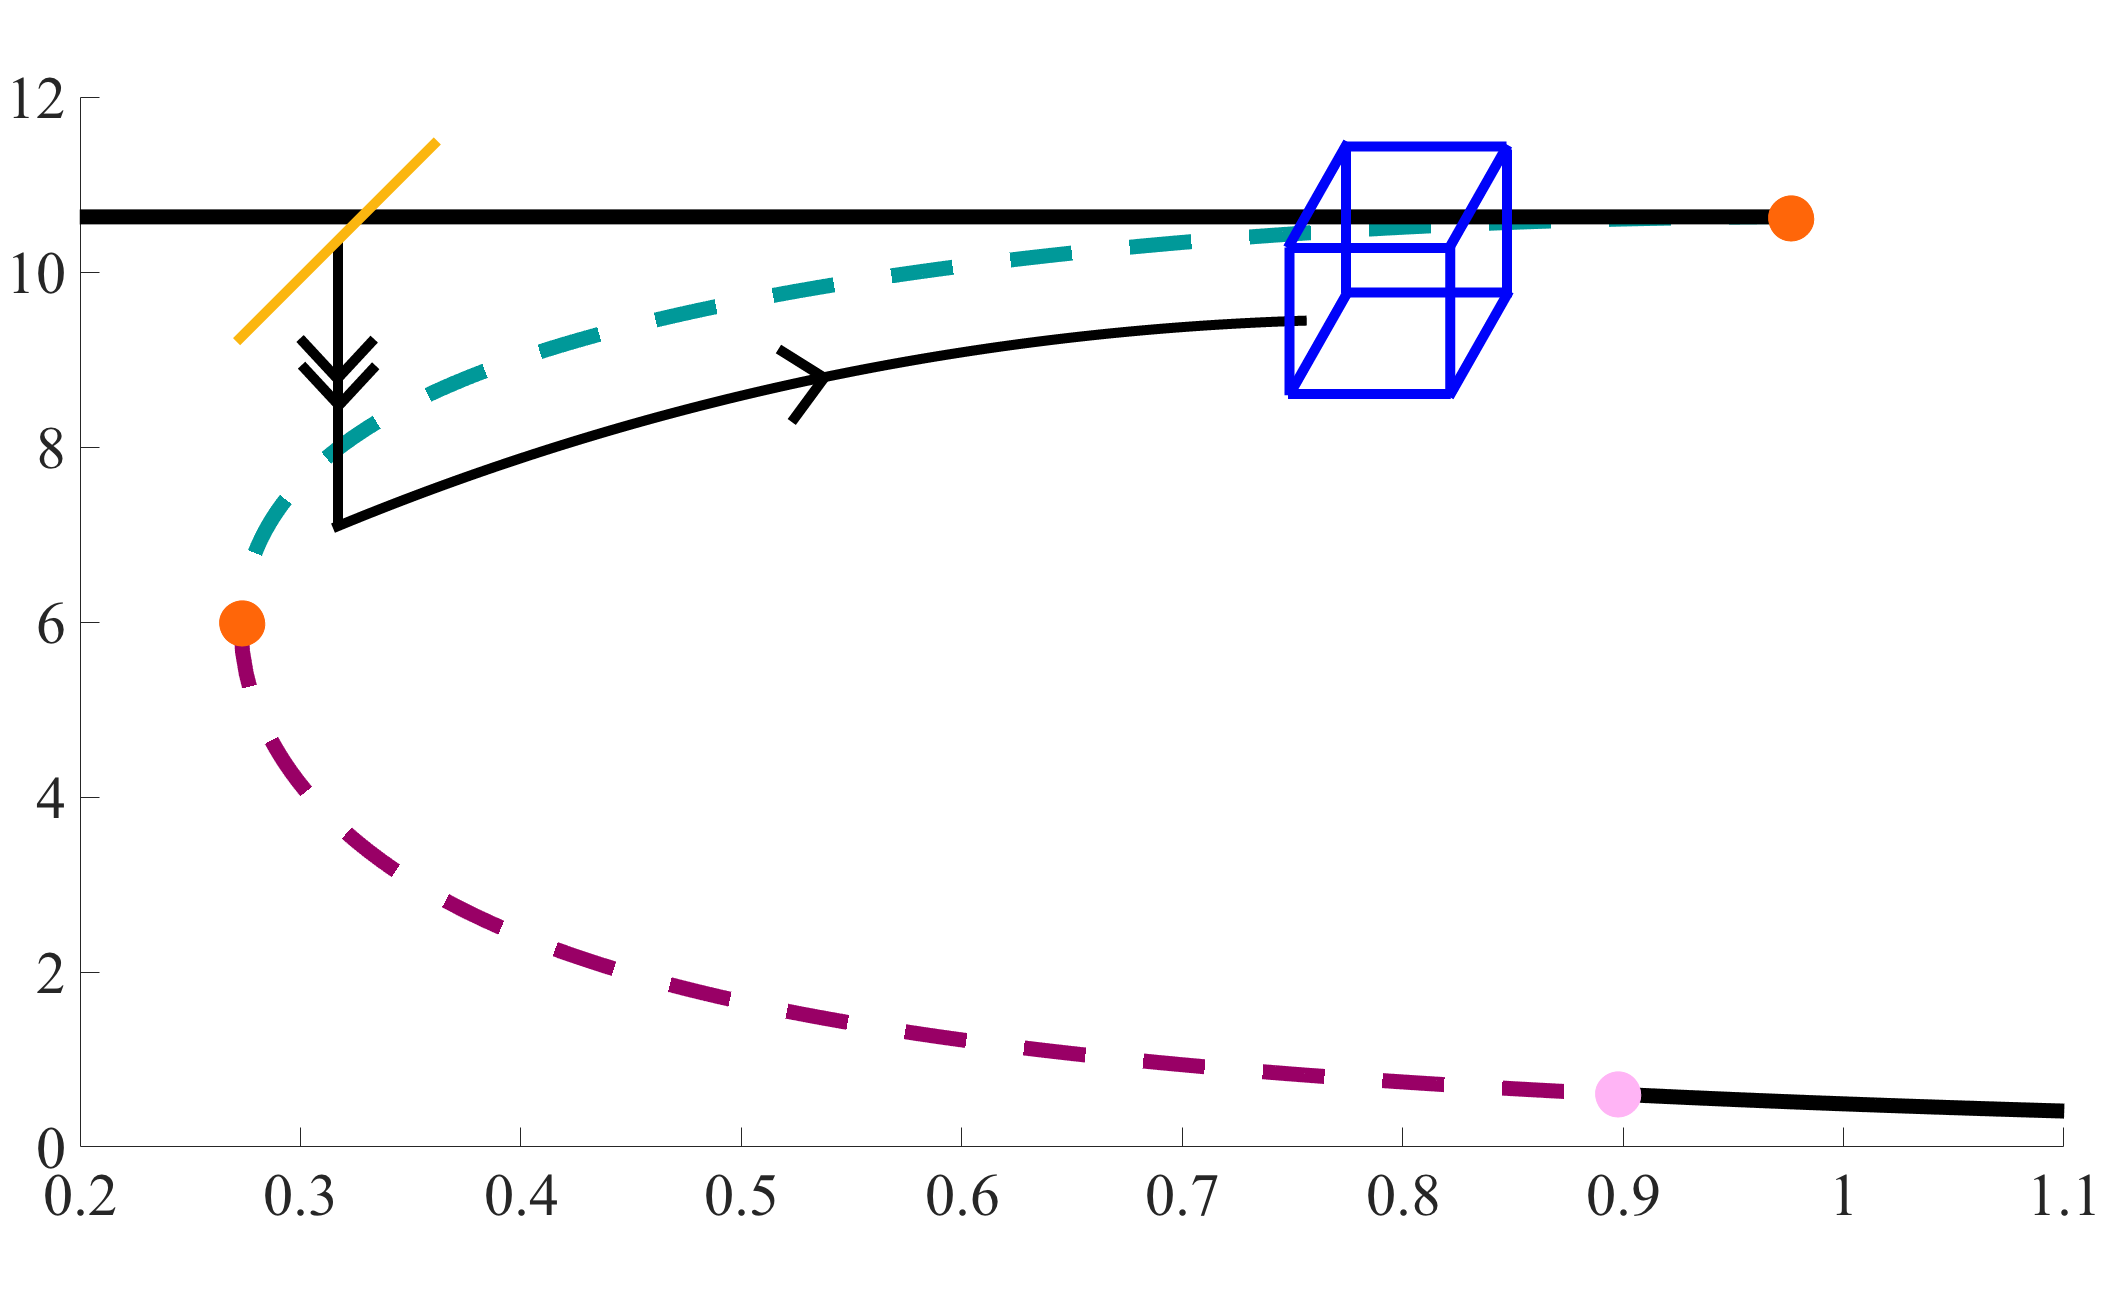
\includegraphics[width=8cm]{./figures_raw/step3.eps}}
 	\put(72,36.5){$\Omega$}
        \put(19,40){$\psi$}
	\put(81,44){$F_1$}
        \put(19,29){$F_2$}
        \put(72.5,13.5){$H$}
        \put(50,46.5){$C^4_+$}
        \put(7,46){$A$}
        \put(80,13){$C^4_-$}
        \put(50,15){$C^2$}
        \put(50,38.5){$\mathbf{u}$} 
        \put(26.5,42){$\mathbf{u}(0)$}       
        \put(6,39){\footnotesize $9.0$}
        \put(6,19){\footnotesize $3.0$}
	\put(24.5,7.5){\footnotesize $0.3$}
	\put(40.4,7.5){\footnotesize $0.5$}
	\put(56.4,7.5){\footnotesize $0.7$}
	\put(72.2,7.5){\footnotesize $0.9$}
	\put(86,6.9){$B$}
	\put(13,13.5){(c)}
	\put(25,20){$q$}
	\end{picture}
	}
\put(89,0){\begin{picture}(85,43)(5,7)
	\put(10.25,10){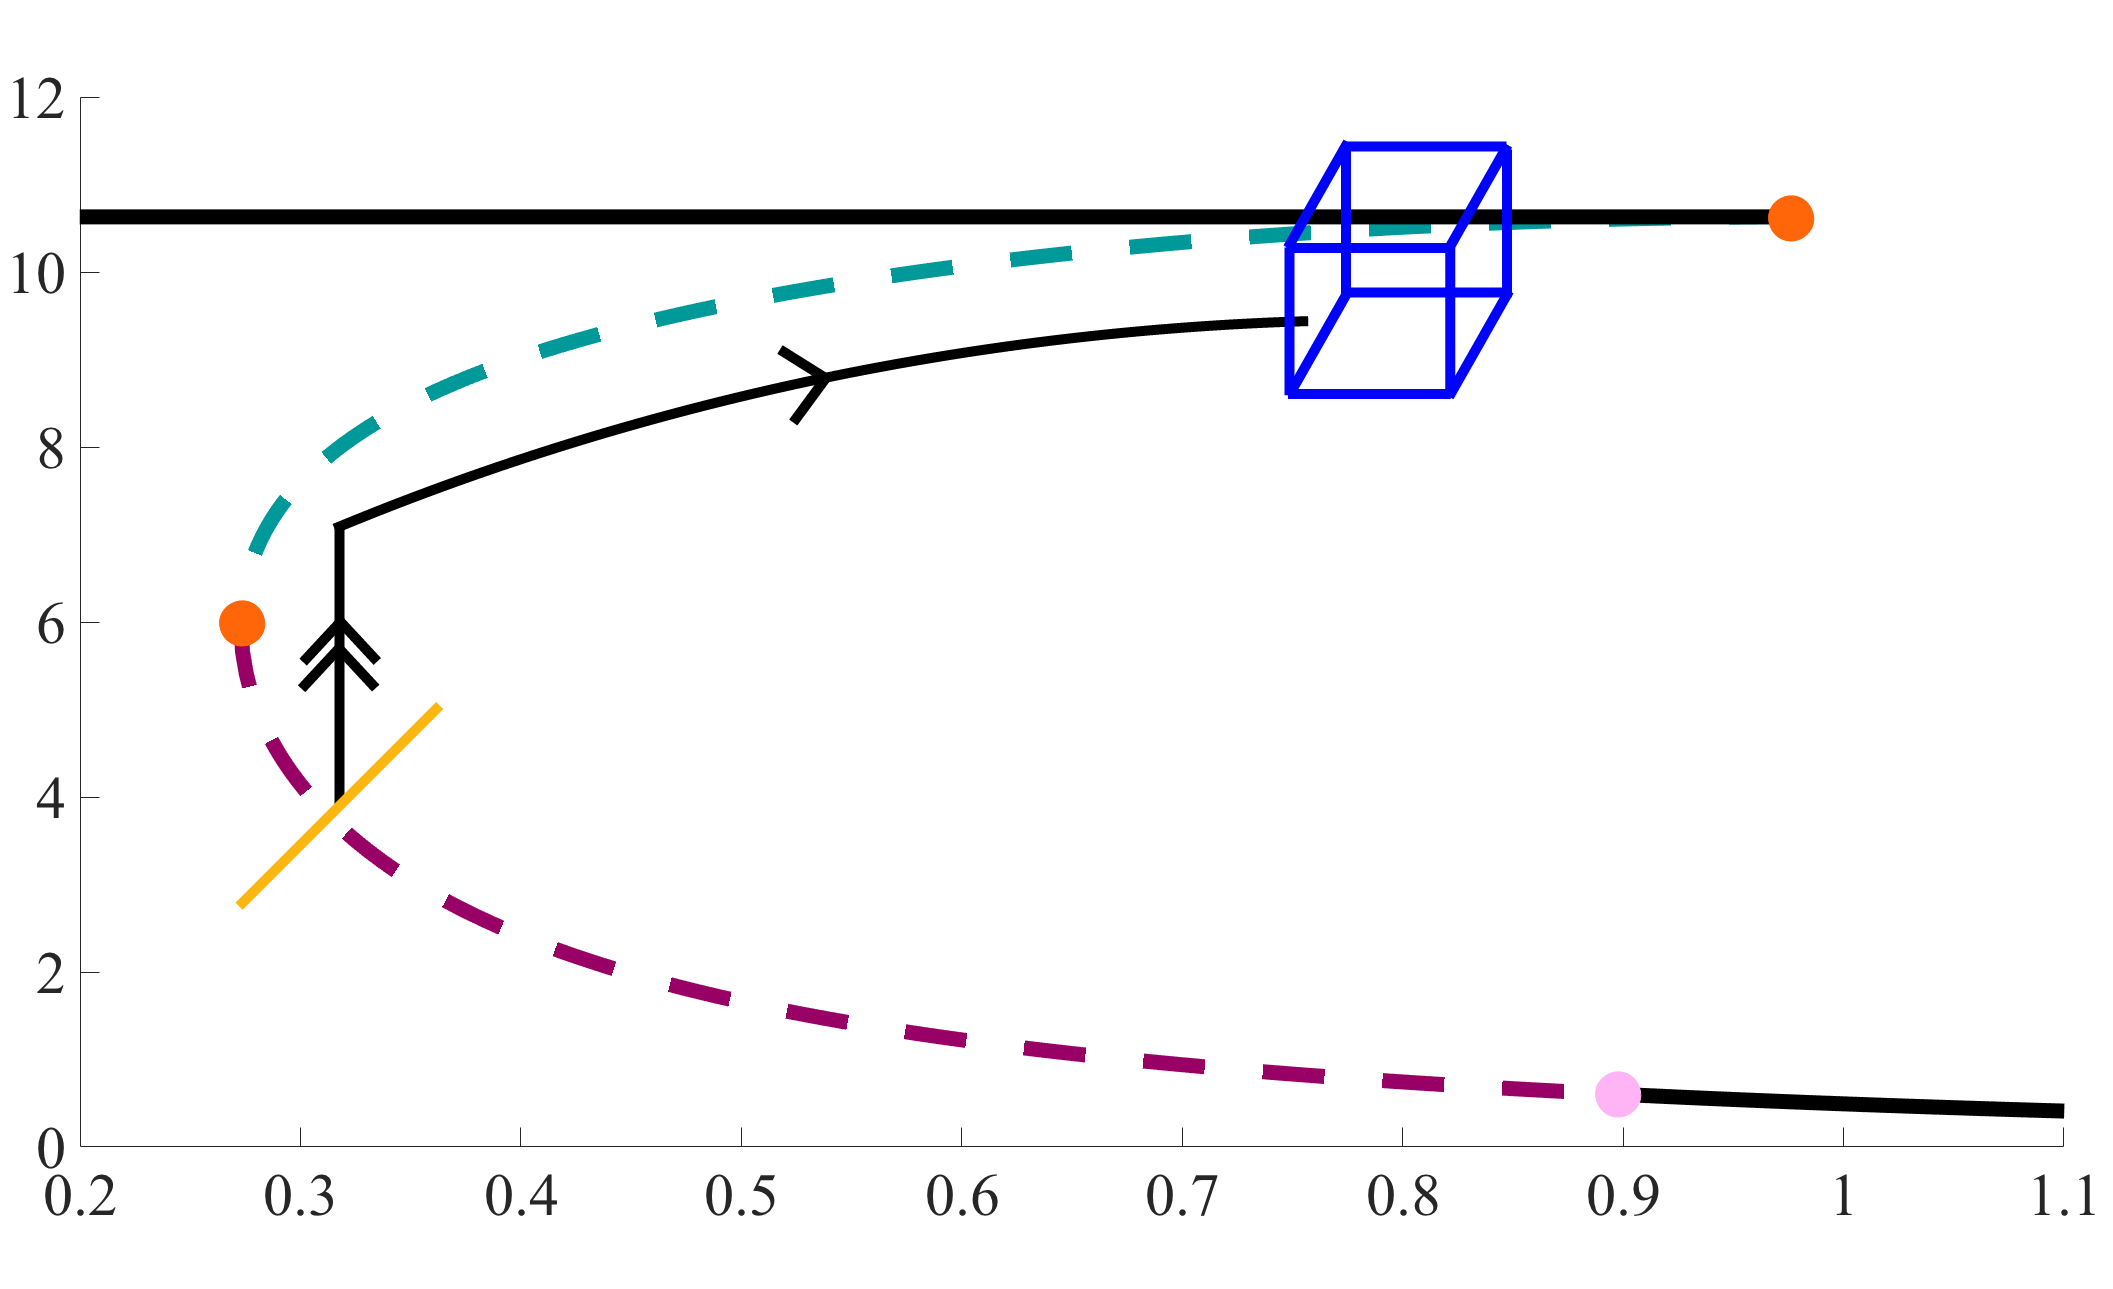
\includegraphics[width=8cm]{./figures_raw/step4.eps}}
	\put(72,36.5){$\Omega$}
        \put(33,20){$\psi$}
	\put(81,44){$F_1$}
        \put(19,29){$F_2$}
        \put(72.5,13.5){$H$}
        \put(7,46){$A$}
        \put(50,15){$C^2$}
        \put(80,13){$C^4_-$}   
        \put(50,46.5){$C^4_+$}
        \put(50,38.5){$\mathbf{u}$} 
        \put(30.5,25){$\mathbf{u}(0)$}        
        \put(6,39){\footnotesize $9.0$}
        \put(6,19){\footnotesize $3.0$}
	\put(24.5,7.5){\footnotesize $0.3$}
	\put(40.4,7.5){\footnotesize $0.5$}
	\put(56.4,7.5){\footnotesize $0.7$}
	\put(72.2,7.5){\footnotesize $0.9$}
	\put(86,6.9){$B$}
	\put(13,13.5){(d)}
	\put(25,20){$q$}
	\end{picture}
	\caption{}
}
\end{picture}
\end{figure}

\newpage

%%%%%%%%%%%%%%%%%%%%%%%%%%%
%%% Figure 4: One piece of the stable manifold %%%
%%%%%%%%%%%%%%%%%%%%%%%%%%%

\begin{figure}
\begin{picture}(134,179)(47.5,59.5)
\put(50,140){
	\begin{picture}(180,100)(0,0)
	    \put(0,0){\includegraphics[width=12.6cm]{./figures_raw/one_piece_paper_BAX.png}}
	    \put(115,65){$W^{s}_{\Sigma_0}$}
	    \put(120,24){$\Sigma_0$}
	    \put(-0.75,6){$\Omega$}
	    \put(96,47){$\mathbf{u}$}
	    \put(101,94){$C^3$}
	    \put(70,3){$C^{4}_{+}$}
	    \put(13,81){(a)}
	\end{picture}
	\caption{}
}

\put(50,58){
	\begin{picture}(180,100)(0,0)
	    \put(0,0){\includegraphics[width=12.6cm]{./figures_raw/one_piece_paper_BAY.png}}
	    \put(123,46){$W^{s}_{\Sigma_0}$}
	    \put(-3,5.5){$\Omega$}
	    \put(108,79.5){$C^3$}
	    \put(70,3){$C^{4}_{+}$}
	    \put(102,30){$\mathbf{u}$}
	    \put(123,4.5){$\Sigma_0$}
	    \put(13,60){(b)}
	\end{picture}
	\caption{}
}
\end{picture}
\end{figure}


\newpage



%%%%%%%%%%%%%%%%%%%%%%%%%%%%
%%% Figure 5: Two pieces of the stable manifold %%%
%%%%%%%%%%%%%%%%%%%%%%%%%%%%

\begin{figure}
\begin{picture}(121,170.5)(57,62.5)
\put(50,140){
	\begin{picture}(180,100)(0,0)
	    \put(0,0){\includegraphics[width=12.6cm]{./figures_raw/two_pieces_paper_BAX.eps}}
	    \put(110,50.5){$W^{s}_{\Sigma_0}$}
	    \put(121,32){$\Sigma_0$}
	    \put(13,62){$\Sigma_1$}
	    \put(47.5,5){$\Omega$}
	    \put(30,83){$C^2$}
	    \put(93,54){$C^3$}
	    \put(94,64){$F_2$}
	    \put(88,9){$C^{4}_{+}$}
	    \put(50,44){$\mathbf{u}$}
	    \put(105,37.5){$\mathbf{u}$}	    
	    \put(13,83){(a)}
	\end{picture}
	\caption{}
}

\put(50,60){
	\begin{picture}(180,100)(0,0)
	    \put(0,2){\includegraphics[width=12.6cm]{./figures_raw/two_pieces_paper_BAY.eps}}
	    \put(110,39.5){$W^{s}_{\Sigma_0}$}
	    \put(13,27){$\Sigma_1$}
	    \put(47.25,7){$\Omega$}
	    \put(82.5,60){$C^2$}
	    \put(92,45){$C^3$}
	    \put(88,12){$C^{4}_{+}$}
	    \put(122,22.5){$\Sigma_0$}
	    \put(94.5,54){$F_2$}
	    \put(46,39){$\mathbf{u}$}
	    \put(105,28){$\mathbf{u}$}		    	    
	    \put(13,60){(b)}
	\end{picture}
	\caption{}
}
\end{picture}
\end{figure}


\newpage


%%%%%%%%%%%%%%%%%%%%%%%%%%%%
%%% Figure 6: Five pieces of the stable manifold %%%
%%%%%%%%%%%%%%%%%%%%%%%%%%%%

\begin{figure}
\begin{picture}(120,196)(58,36.5)
\put(50,140){
	\begin{picture}(180,100)(0,0)
	    \put(0,0){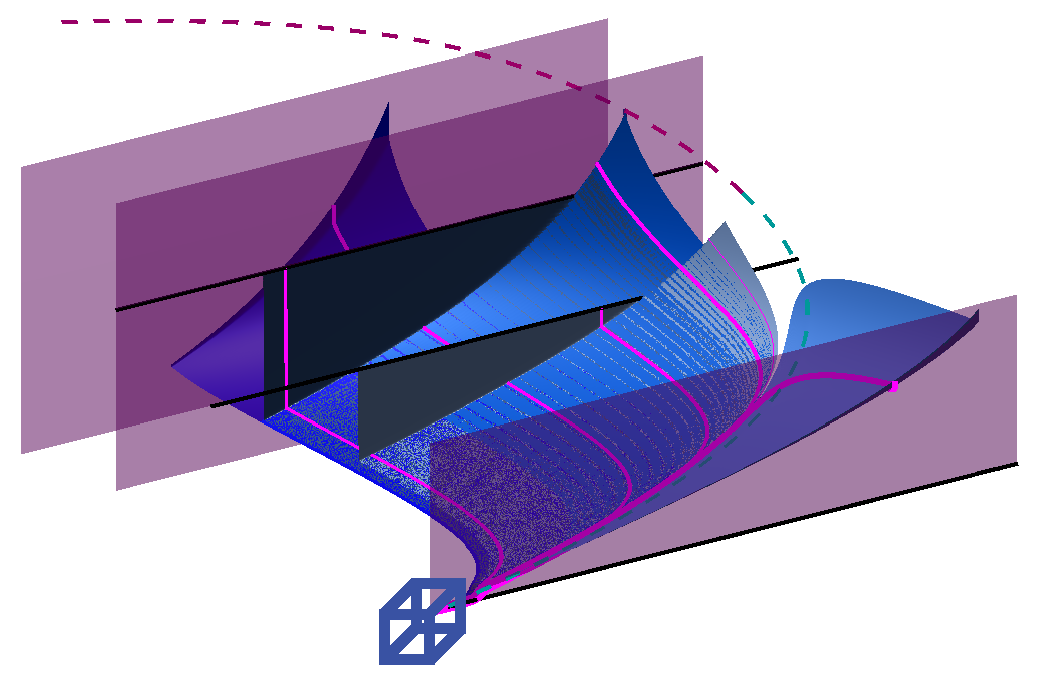
\includegraphics[width=12.6cm]{./figures_raw/five_pieces_paper_BAX.eps}}
	    \put(110,51){$W^{s}_{\Sigma_0}$}
	    \put(121,35){$\Sigma_0$}
	    \put(13,62){$\Sigma_1$}
	    \put(22,57){$\Sigma_2$}
	    \put(24,46.5){$\Sigma_3$}
	    \put(27,30){$\Sigma_4$}
	    \put(48.25,5){$\Omega$}
	    \put(94,64){$F_2$}
	    \put(30,83){$C^2$}
	    \put(99,56){$C^3$}
	    \put(88,9.75){$C^{4}_{+}$}
	    \put(13,83){(a)}
	\end{picture}
	\caption{}
}

\put(50,35){
	\begin{picture}(180,100)(0,0)
	    \put(0,0){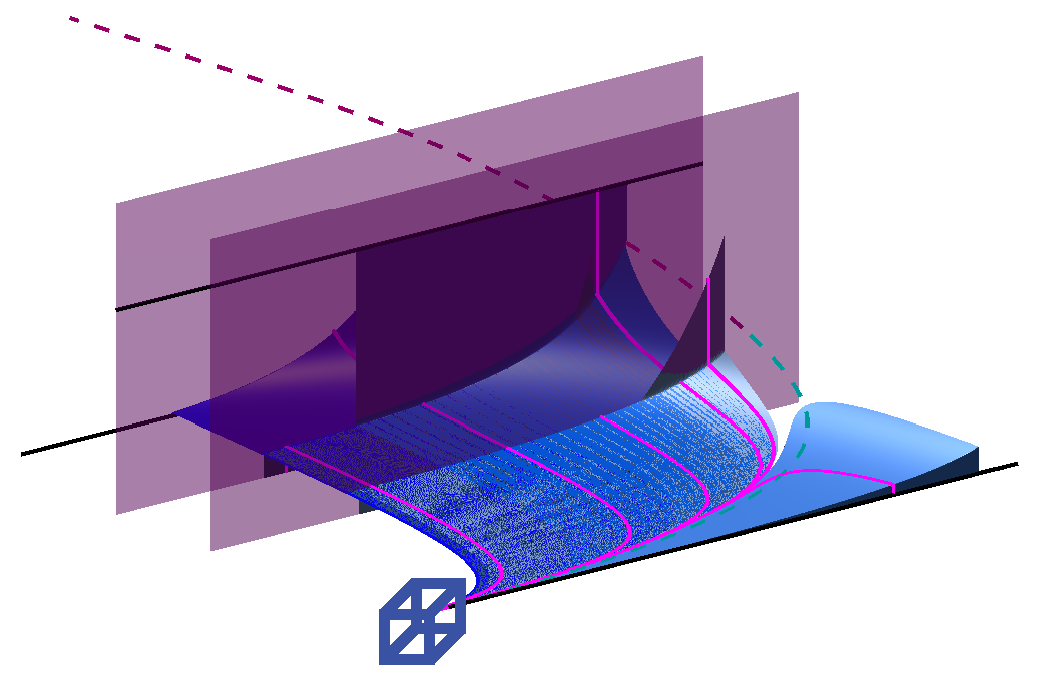
\includegraphics[width=12.6cm]{./figures_raw/five_pieces_paper_BAY.eps}}
	    \put(110,38.5){$W^{s}_{\Sigma_0}$}
	    \put(13,26){$\Sigma_1$}
	    \put(23,72){$\Sigma_2$}
	    \put(22,53){$\Sigma_3$}
	    \put(33,65){$\Sigma_4$}
	    \put(48,6){$\Omega$}
	    \put(56.5,90){$C^2$}
	    \put(98.5,45){$C^3$}
	    \put(88,11.5){$C^{4}_{+}$}
	    \put(94.5,54){$F_2$}
	    \put(122,21){$\Sigma_0$}
	    \put(13,81){(b)}
	\end{picture}
	\caption{}
}
\end{picture}
\end{figure}
\newpage

%%%%%%%%%%%%%%%%%%%%%%%%%%%%
%%% Figure 7: unstable manifold numerical set up %%%
%%%%%%%%%%%%%%%%%%%%%%%%%%%%

\begin{figure}
\begin{picture}(172.75,30.5)(2,-0.5)
\put(0,0){
	\begin{picture}(85,43)(5,7)
	\put(10.25,10){\includegraphics[width=8cm]{./figures_raw/unstable_step1.eps}}
        \put(83,20.5){$\Phi$}
        \put(39.5,16){$\chi$}        
        \put(72.25,15.25){$H$}
        \put(28,24.5){$C^2$}
        \put(7.5,33){$A$}
        \put(6,22.25){\footnotesize $4.0$}
	\put(24.5,7.5){\footnotesize $0.3$}
	\put(40.4,7.5){\footnotesize $0.5$}
	\put(56.4,7.5){\footnotesize $0.7$}
	\put(72.2,7.5){\footnotesize $0.9$}
	\put(86,6.9){$B$}
	\put(13,13.5){(a)}
	\put(25.5,30.5){$q$}
	\end{picture}
	\caption{}
	}

\put(88,0){
	\begin{picture}(85,43)(5,7)
	\put(10.25,10){\includegraphics[width=8cm]{./figures_raw/unstable_step2.eps}}
        \put(34.5,14){$\Theta$}
        \put(81.5,19){$\Phi_{\widehat{B}}$}
        \put(41.25,29){$\mathbf{w}(1)$}
        \put(28,24.5){$C^2$}
        \put(7.75,33){$A$}
        \put(6.5,22.25){\footnotesize $4.0$}
	\put(24.5,7.5){\footnotesize $0.3$}
	\put(40.4,7.5){\footnotesize $0.5$}
	\put(56.4,7.5){\footnotesize $0.7$}
	\put(72.2,7.5){\footnotesize $0.9$}
	\put(86,6.9){$B$}
	\put(13,13.5){(a)}
	\put(25.5,30.5){$q$}

	\end{picture}
	\caption{}
	}
\end{picture}
\end{figure}

\newpage



%%%%%%%%%%%%%%%%%%%%%%%%%%%
%%% Figure 8: One piece of the unstable manifold %%
%%%%%%%%%%%%%%%%%%%%%%%%%%%
\begin{figure}
\begin{picture}(131,142.5)(99.5,104.5)
\put(100,160){
	\begin{picture}(180,100)(0,0)
	    \put(0,24){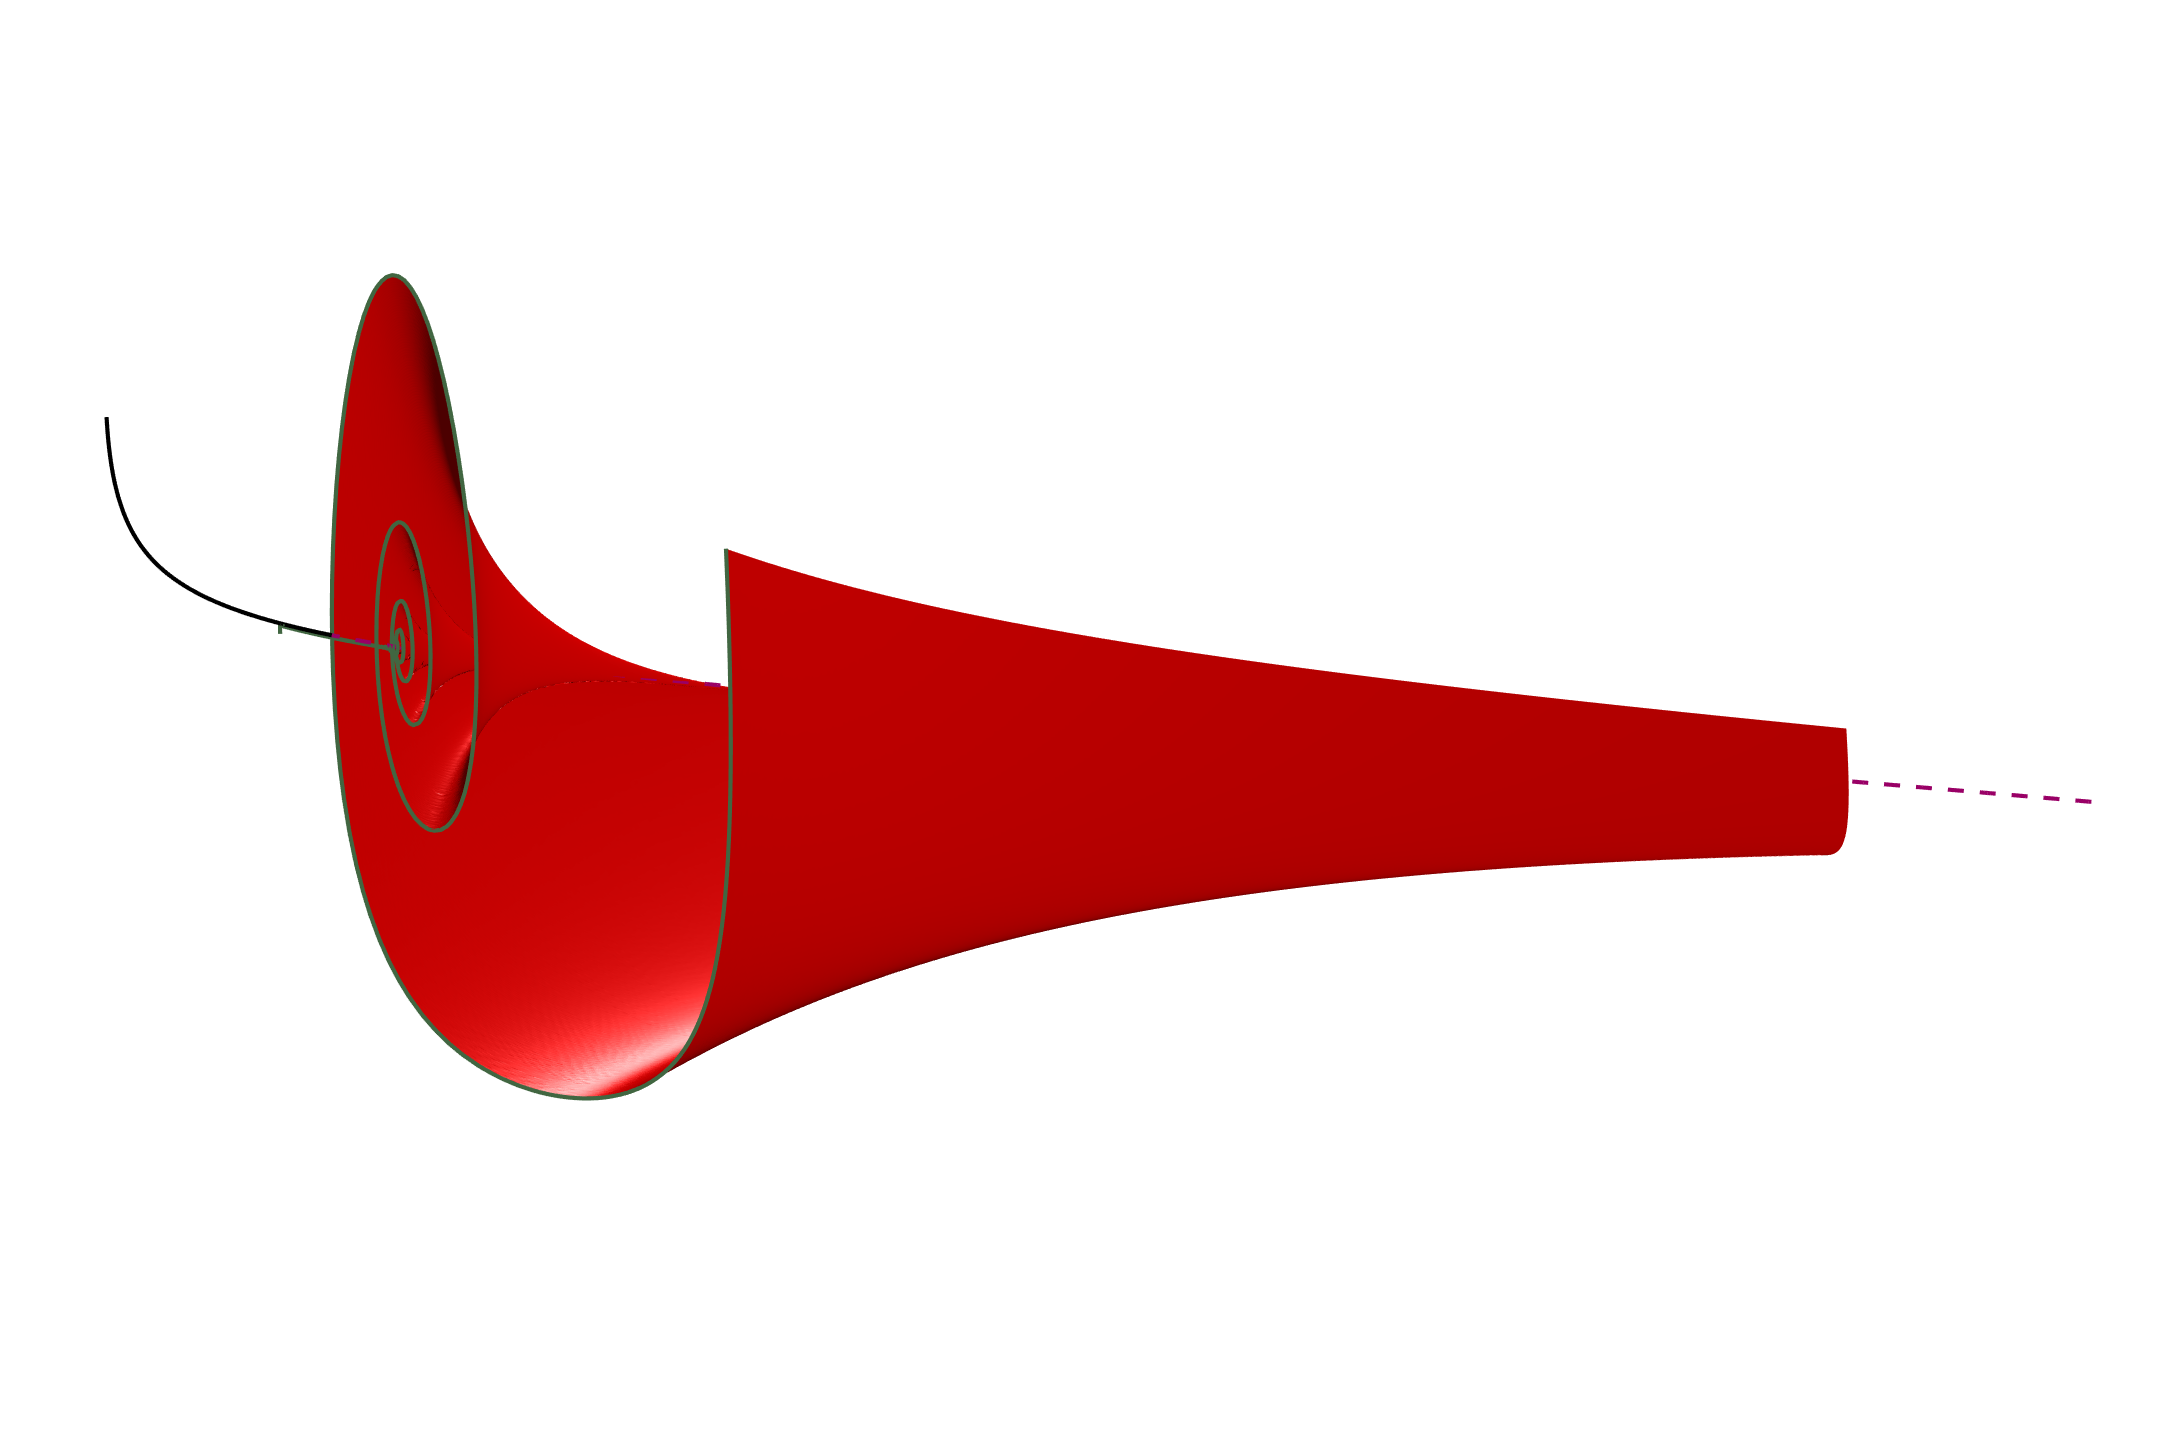
\includegraphics[width=12.6cm]{./figures_raw/unstable_piece_BAX.eps}}
	    \put(70,59.5){$W^{u}_{r}\cap\mathscr{D}^u$}
	    \put(70,36){$W^{u}_{r}$}
	    \put(11,69.5){$\Phi_{\widehat{B}}$}
	     \put(15,55){$H$}
	    \put(0,70){$C^4_-$}
	    \put(118,49){$C^2$}
	    \put(2,81){(a)}
	\end{picture}
	\caption{}
}

\put(100,85){
	\begin{picture}(180,100)(0,0)
	    \put(3,19.5){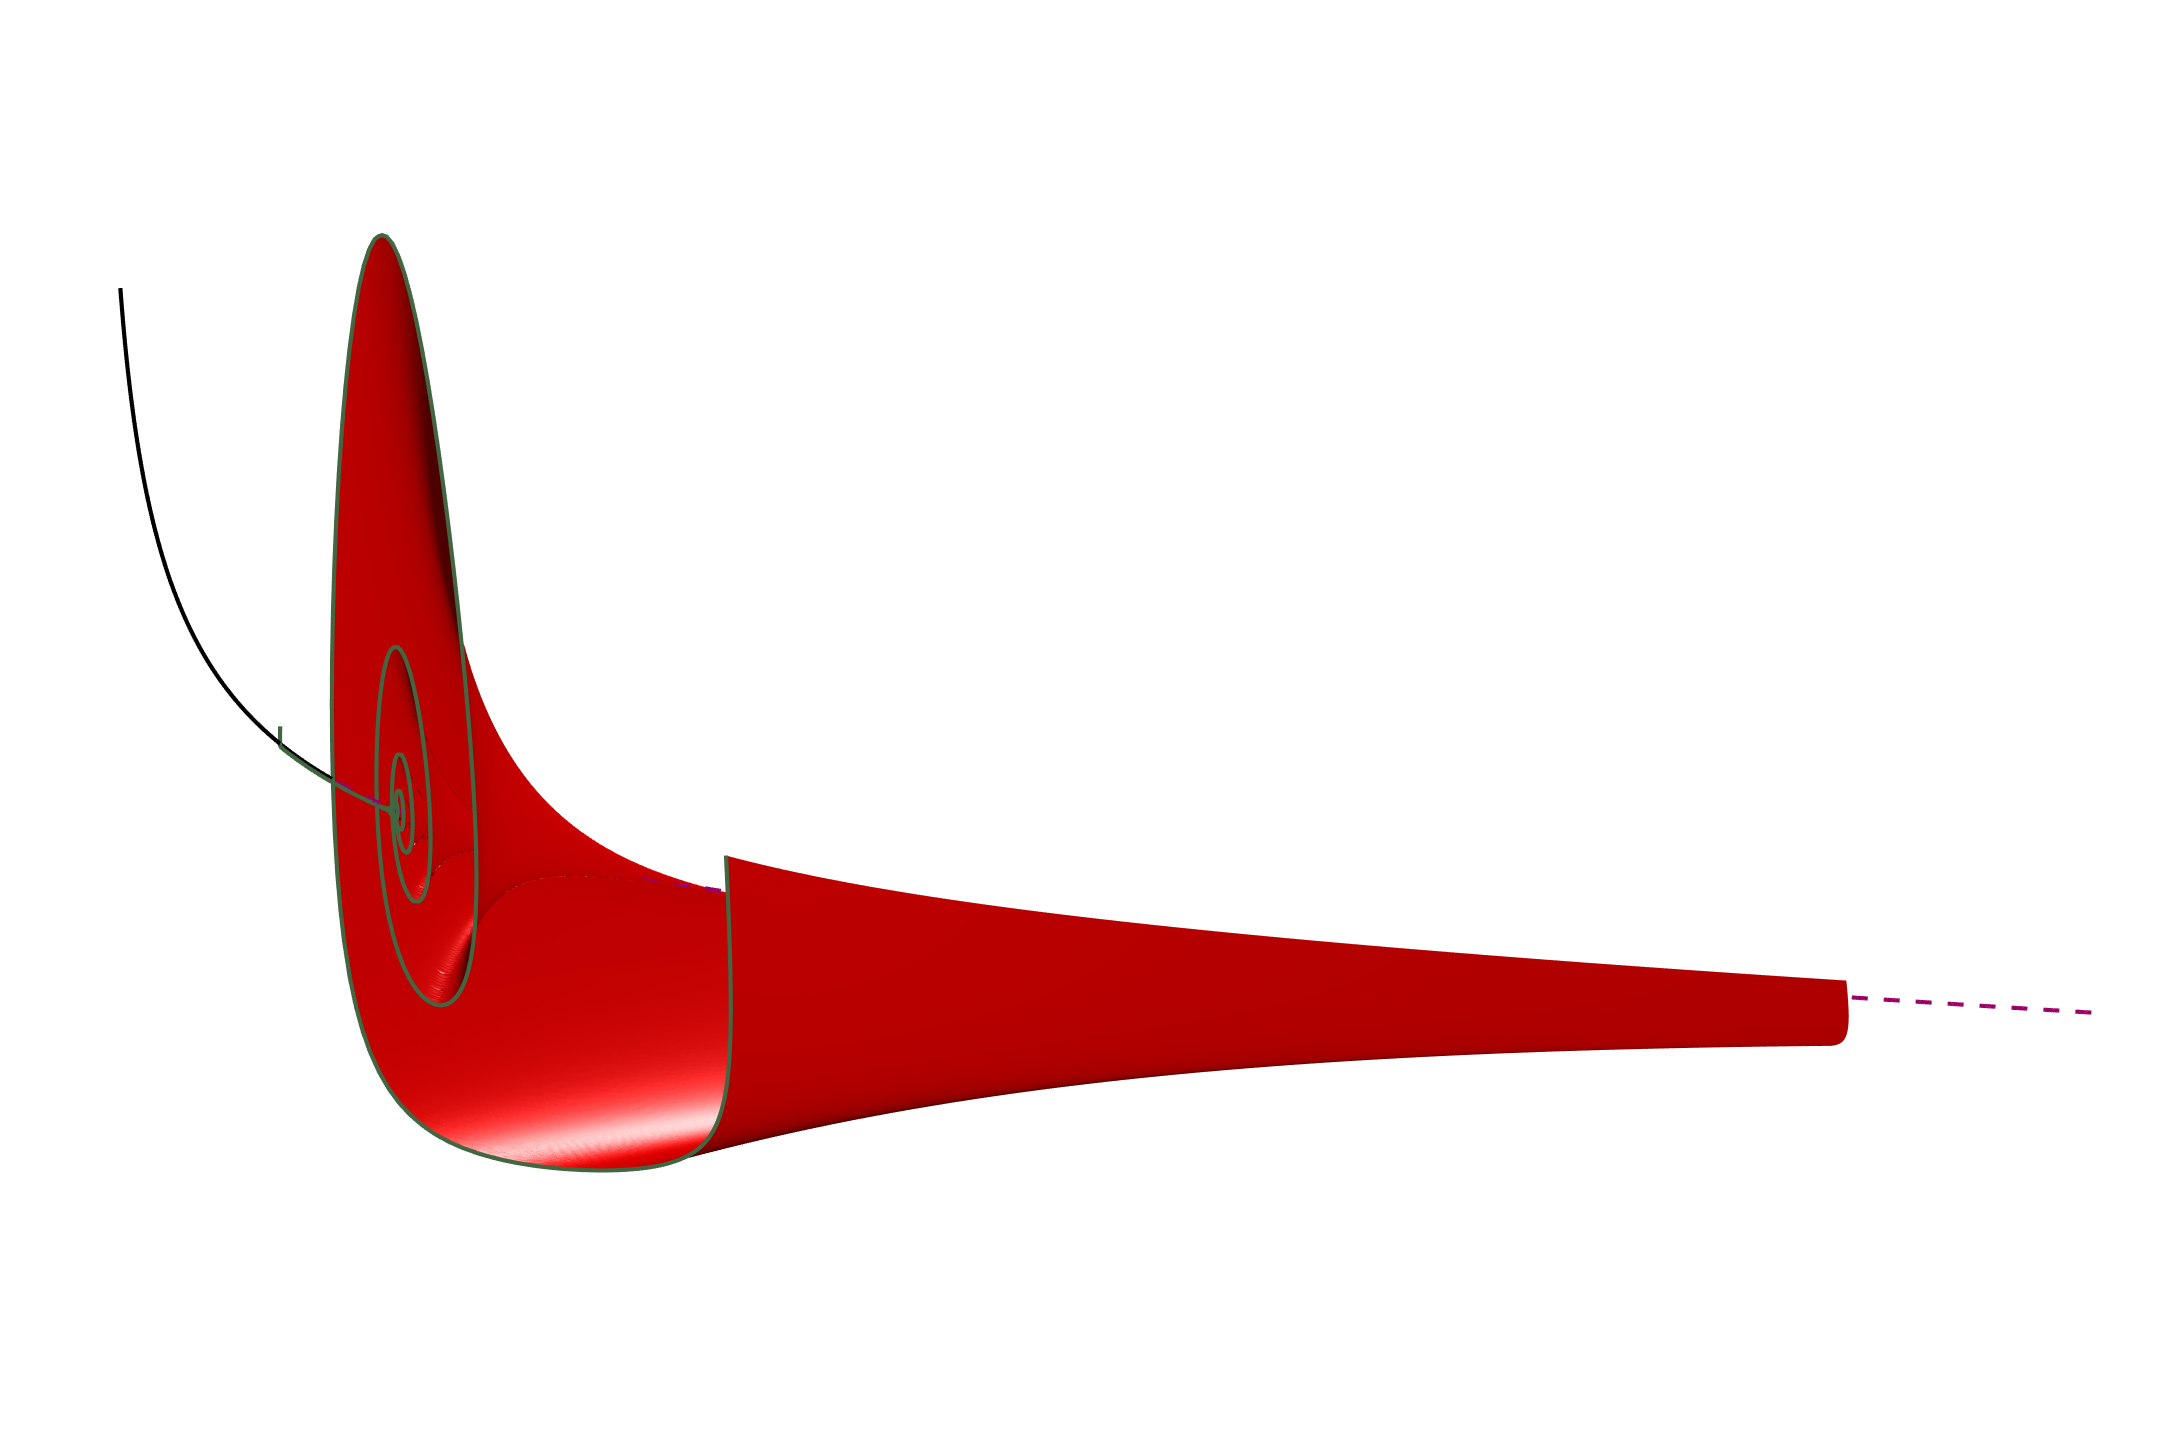
\includegraphics[width=12.6cm]{./figures_raw/unstable_piece_BAY.eps}}
	    \put(70,40){$W^{u}_{r}\cap\mathscr{D}^u$}
	    \put(70,23.5){$W^{u}_{r}$}
	    \put(13.75,62){$\Phi_{\widehat{B}}$}	    
	    \put(14,62.5){$$}
	    \put(18,45){$H$}
	    \put(4.5,73){$C^4_-$}
	    \put(118,34){$C^2$}
	    \put(2,87){(b)}
	\end{picture}
	\caption{}
}
\end{picture}
\end{figure}

%%%%%%%%%%%%%%%%%%%%%%%%%%%
%%% Figure 9: Almost heteroclinic connection    %%
%%%%%%%%%%%%%%%%%%%%%%%%%%%
\begin{figure}
\begin{picture}(131,165)(99.5,113)
\put(100,173.5){
	\begin{picture}(180,100)(0,0)
	    \put(0,24){\includegraphics[width=12.6cm]{./figures_raw/almost_hetclin_BAX.eps}}
	    \put(6.5,72){$H$}
	    \put(2,78){$C^4_-$}
	    \put(118,33.5){$C^4_+$}
	    \put(106,49){$C^3$}
	    \put(98.5,61.25){$F_2$}
	    \put(2,91){(a)}
	\end{picture}
	\caption{}
}

\put(100,95.5){
	\begin{picture}(180,100)(0,0)
	    \put(3,19.5){\includegraphics[width=12.6cm]{./figures_raw/almost_hetclin_BAY.eps}}
	    \put(9.5,53.5){$H$}
	    \put(5,61){$C^4_-$}
	    \put(109.5,31){$C^3$}
	    \put(120.5,28.6){$C^4_+$}
	    \put(91,100){$F_1$}
	    \put(94,18){$F_1$}
	    \put(102,37.75){$F_2$}
	    \put(2,87){(b)}
	\end{picture}
	\caption{}
}
\end{picture}
\end{figure}


%%%%%%%%%%%%%%%%%%%%%%%%%%
%%% Figure 10: Lin's method numerical set up %%%
%%%%%%%%%%%%%%%%%%%%%%%%%%

\begin{figure}
\begin{picture}(172.5,45)(0,0)
\put(-1.5,1){
	\begin{picture}(85,43)(5,7)
	\put(10.25,10){\includegraphics[width=8cm]{./figures_raw/Lin3.eps}}
        \put(7,46){$A$}
        \put(49.25,38.5){$\mathbf{u}$}
        \put(65,15.5){$\mathbf{w}$}
        \put(35,26.5){$\eta/Z$}
        \put(48.5,31.5){$\mathbf{w}(1)_B=B_1$}
        \put(6,39){\footnotesize $9.0$}
        \put(6,19){\footnotesize $3.0$}
	\put(24.5,7.5){\footnotesize $0.3$}
	\put(40.4,7.5){\footnotesize $0.5$}
	\put(56.4,7.5){\footnotesize $0.7$}
	\put(72.2,7.5){\footnotesize $0.9$}
	\put(86,6.9){$B$}
	\put(72,37.75){$E^s(p_{\mathrm{out}})$}
	\put(83,15.5){$\Phi_{\widehat{B}}$}
       \put(15,31){$\mathscr{L}$}
	\put(20,41.5){$C^4_+$}
	\put(81,44){$F_1$}
	\put(25,20){$q$}
	\put(13,13.5){(a)}
	\end{picture}
	}
\put(86.5,1){\begin{picture}(85,43)(5,7)
	\put(10.25,10){\includegraphics[width=8cm]{./figures_raw/Lin4.eps}}
	\put(61.25,40){$\mathbf{u}$}
        \put(65,15.5){$\mathbf{w}$}
        \put(7,46){$A$}
        \put(6,39){\footnotesize $9.0$}
        \put(6,19){\footnotesize $3.0$}
	\put(24.5,7.5){\footnotesize $0.3$}
	\put(40.4,7.5){\footnotesize $0.5$}
	\put(56.4,7.5){\footnotesize $0.7$}
	\put(72.2,7.5){\footnotesize $0.9$}
	\put(86,6.9){$B$}
	\put(72,37.75){$E^s(p_{\mathrm{out}})$}
	\put(83,15.5){$\Phi_{\widehat{B}}$}
        \put(15,31){$\mathscr{L}$}
	\put(20,41.5){$C^4_+$}
	\put(25,20){$q$}
	\put(81,44){$F_1$}
	\put(13,13.5){(b)}
	\end{picture}
	\caption{}
}
\end{picture}
\end{figure}

\newpage



%%%%%%%%%%%%%%%%%%%%%%%%%%%%
%% Figure 11: Heteroclinic surface, numerical set up %%
%%%%%%%%%%%%%%%%%%%%%%%%%%%%

\begin{figure}
\begin{picture}(122,173)(52,48.5)
\put(50,140){
	\begin{picture}(180,100)(0,0)
	    \put(0,0){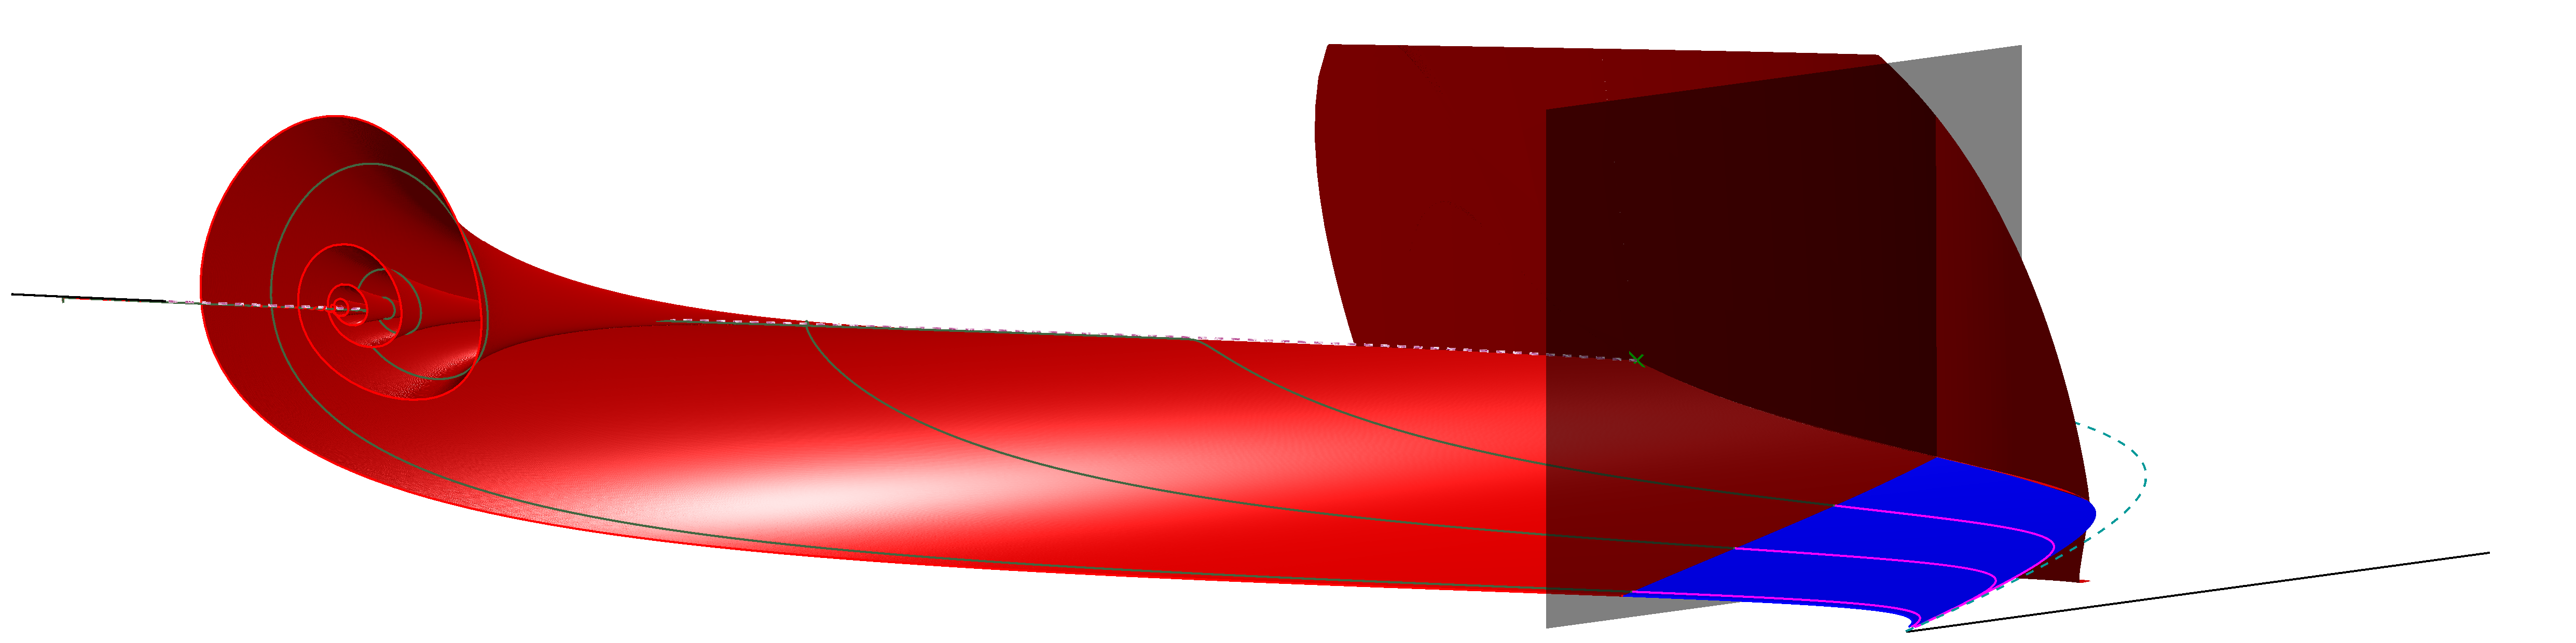
\includegraphics[width=12.6cm]{./figures_raw/hetclin_6_BAX.eps}}
	    \put(92.5,34){$\mathscr{L}$}
	    \put(90,41){$C^2$}
	    \put(105.5,28){$C^3$}
	    \put(108,4.5){$C^{4}_{+}$}
	     \put(2.5,54.5){$C^{4}_{-}$}
	     \put(48,7){$\mathscr{H}$}
	     \put(6.75,48){$H$}
	     \put(79,46){$q$}
	     \put(99,37.5){$F_2$}
	     \put(91,-2){$F_1$}
	    \put(5,77){(a)}
	\end{picture}
	\caption{}
}

\put(50,50){
	\begin{picture}(180,100)(0,0)
	    \put(0,-0.5){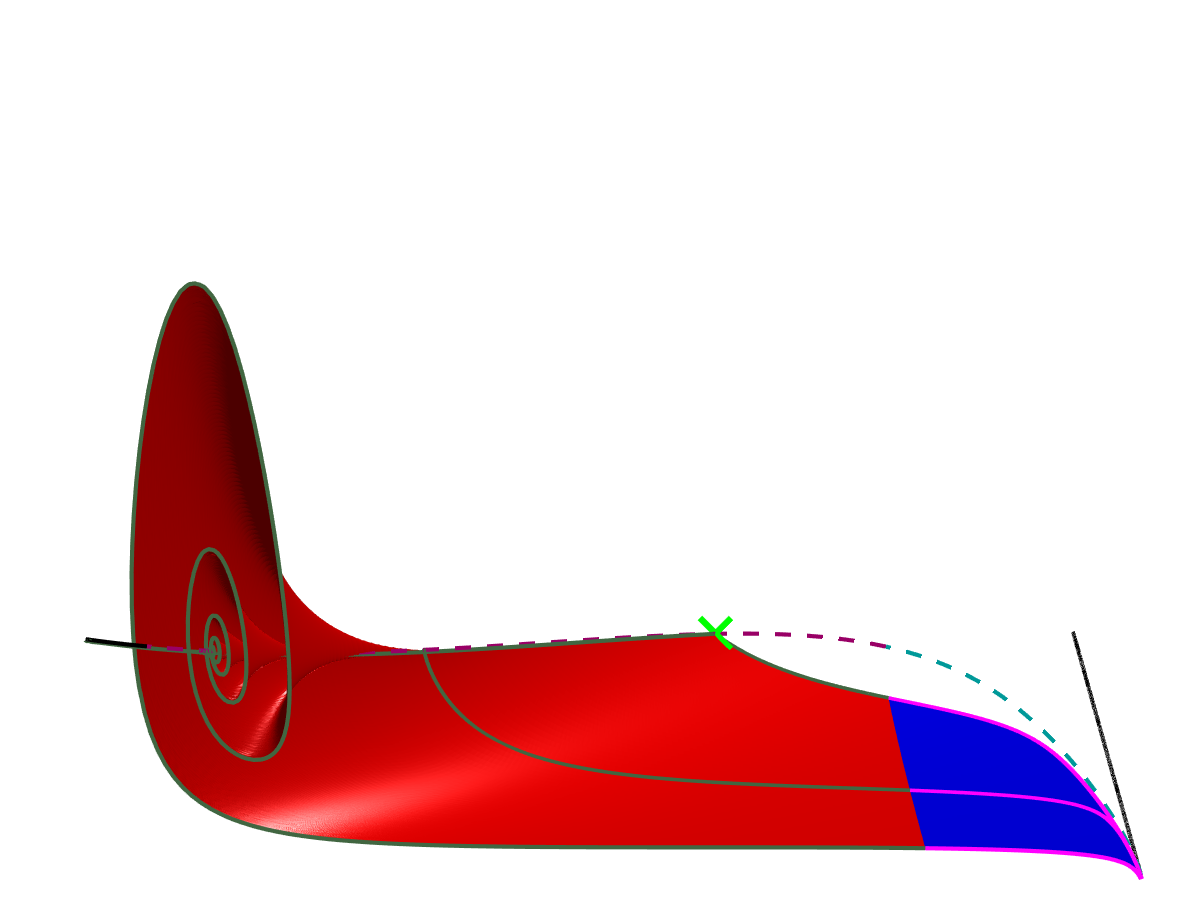
\includegraphics[width=12.6cm]{./figures_raw/hetclin_6_BAY.eps}}
	    \put(92.5,32){$\mathscr{L}$}
	    \put(90,22.5){$C^2$}
	    \put(106,13){$C^3$}
	    \put(108,6.5){$C^{4}_{+}$}
	    \put(2.5,42){$C^{4}_{-}$}
	    \put(48,3){$\mathscr{H}$}
	    \put(6.75,34.5){$H$}
	    \put(79,26.5){$q$}
	    \put(99,20.5){$F_2$}
	    \put(91,-0.5){$F_1$}
	    \put(5,81){(b)}
	\end{picture}
	\caption{}
}
\end{picture}
\end{figure}
\newpage

%%%%%%%%%%%%%%%%%%%%%%%%%%%%%%%%%%%
%% Figure 12: Faded heteroclinic surface with unstable manifold %%
%%%%%%%%%%%%%%%%%%%%%%%%%%%%%%%%%%%

\begin{figure}
\begin{picture}(124,175)(51,69.5)
\put(50,162){
	\begin{picture}(180,100)(0,0)
	    \put(0,0){\includegraphics[width=12.6cm]{./figures_raw/paper_saddle_unstable_BAX.eps}}
	    \put(91,72){$W^u(q)$}
	    \put(105.5,28){$C^3$}
	    \put(108,4.5){$C^{4}_{+}$}
	    \put(91,-1){$F_1$}
	     \put(2.5,54.5){$C^{4}_{-}$}
	      \put(6.75,48){$H$}
	     \put(48,7){$\mathscr{H}$}
	     \put(81,43.5){$q$}
	    \put(5,77){(a)}
	\end{picture}
	\caption{}
}

\put(50,71.5){
	\begin{picture}(180,100)(0,0)
	    \put(0,0){\includegraphics[width=12.6cm]{./figures_raw/paper_saddle_unstable_BAY.eps}}
	    \put(87,51){$W^u(q)$}
	    \put(105.5,13){$C^3$}
	    \put(108,4.5){$C^{4}_{+}$}
	    \put(2.5,41.5){$C^{4}_{-}$}
	    \put(6.75,34){$H$}
	    \put(48,1.5){$\mathscr{H}$}
	    \put(91,-1){$F_1$}
	    \put(81,23){$q$}
	    \put(5,81){(b)}
	\end{picture}
	\caption{}
}
\end{picture}
\end{figure}
\newpage

%%%%%%%%%%%%%%%%%%%%%%%%%%%%%%%%%%%%%%
%% Figure 13: Compare non-singular with singular heteroclinic surface %%
%%%%%%%%%%%%%%%%%%%%%%%%%%%%%%%%%%%%%%

\begin{figure}
\begin{picture}(124,169)(51,53)
\put(50,140){
	\begin{picture}(180,100)(0,0)
	    \put(0,0){\includegraphics[width=12.6cm]{./figures_raw/paper_singular_BAX.eps}}
	    \put(90,41){$C^2$}
	     \put(81.5,45){$q$}
	    \put(105.5,28){$C^3$}
	    \put(99.5,37.5){$F_2$}
	    \put(108,4.5){$C^{4}_{+}$}
	    \put(91,-1){$F_1$}
	     \put(2.5,54.5){$C^{4}_{-}$}
	      \put(6.75,48){$H$}
	     \put(48,7){$\mathscr{H}_0$}
	    \put(5,77){(a)}
	\end{picture}
	\caption{}
}

\put(50,55){
	\begin{picture}(180,100)(0,0)
	    \put(0,0){\includegraphics[width=12.6cm]{./figures_raw/paper_BAX.eps}}
 \put(90,41){$C^2$}
	     \put(81.5,45){$q$}
	    \put(105.5,28){$C^3$}
	    \put(99.5,37.5){$F_2$}
	    \put(108,4.5){$C^{4}_{+}$}
	    \put(91,-1){$F_1$}
	     \put(2.5,54.5){$C^{4}_{-}$}
	      \put(6.75,48){$H$}
	     \put(48,7){$\mathscr{H}$}
	    \put(5,75){(b)}
	\end{picture}
	\caption{}
}
\end{picture}
\end{figure}
\newpage


%%%%%%%%%%%%%%%%%%%%%%%%%
%%%% Figure 17: MMO surface interaction %%%
%%%%%%%%%%%%%%%%%%%%%%%%%

\begin{figure}
\begin{picture}(130,111.6)(64,137.5)
\put(50,140){
	\begin{picture}(180,100)(0,0)
	    \put(0,0){\includegraphics[width=15.12cm]{./figures_raw/MMO_surface_interaction_BAX.eps}}
	    \put(136,16.5){$C^2$}
	    \put(128,5){$C^3$}
	    \put(130,97){(b)}
	    \put(115,50){$\mathscr{H}$}
	    \put(75,0){$C^{4}_{+}$}
	    \put(16,1){$F_1$}
	    \put(27,22){$C^{4}_{-}$}
	    \put(92,23.5){$\mathscr{H}$}
	    \put(20,70){$\Gamma$}
	    \put(20,100){(a)}
	    \put(138.5,10.5){$F_2$}
	\end{picture}
	\caption{}
}
\end{picture}
\end{figure}
\newpage

%%%%%%%%%%%%%%%%%%%%%%%%%%%%%%%%%%%%%%
%%%%%%%%%%%% Figure 13: isola%%%%%%%%%%%%%%%%%%
%%%%%%%%%%%%%%%%%%%%%%%%%%%%%%%%%%%%%%

\begin{figure}
\begin{picture}(124,131)(51,53)
\put(50,120){
\begin{picture}(124,64.5)(86.5,96.5)
	    \put(100,100){\includegraphics[width=11cm]{./figures_raw/paper_isola.eps}}
	    \put(87,157){max($A$)}
	    \put(89,139){\footnotesize $10.3667$}
	    \put(89,119){\footnotesize $10.1333$}
            \put(207,96.75){\Large $\varepsilon$}
            \put(120.5,97){\footnotesize$1.1E-3$}
            \put(144.5,97){\footnotesize$1.9E-3$}
            \put(167.5,97){\footnotesize$2.7E-3$}
            \put(190.5,97){\footnotesize$3.5E-3$}
            \put(197,155){[a]}
            \put(104,137.5){[b]}
            \put(197,110){[c]}
            \put(204,155.5){(a)}
            
	\end{picture}

	\caption{}
}

\put(50,55){
	\begin{picture}(124,64.5)(86.5,96.5)
	    \put(100,100){\includegraphics[width=11cm]{./figures_raw/paper_isola_period.eps}}
	    \put(95,157){$T_\Gamma$}
	    \put(96.5,139){\footnotesize $95$}
	    \put(96.5,119){\footnotesize $85$}
            \put(207,96.75){\Large $\varepsilon$}
            \put(120.5,97){\footnotesize$1.1E-3$}
            \put(144.5,97){\footnotesize$1.9E-3$}
            \put(167.5,97){\footnotesize$2.7E-3$}
            \put(190.5,97){\footnotesize$3.5E-3$}
            \put(202,125.5){[c]}
            \put(101.5,156){[b]}
            \put(196.5,106){[a]}
            \put(204,155.5){(b)}            
	\end{picture}

	\caption{}
}
\end{picture}
\end{figure}
\newpage


%%%%%%%%%%%%%%%%%%%%%%%%%%%%%%%%%%%%%
%%%%%%% Figure 19: Compare MMOs and singular objects%%%%%%
%%%%%%%%%%%%%%%%%%%%%%%%%%%%%%%%%%%%%

\begin{figure}
\begin{picture}(160,192)(76,81)


\put(50,163){
	\begin{picture}(180,100)(0,0)
	    \put(0,0){\includegraphics[width=12.6cm]{./figures_raw/MMO_2_BAX.eps}}
	    \put(70,-2){$C^{4}_{+}$}
	     \put(26,16){$C^{4}_{-}$}
	     \put(90,18){$\mathscr{H}_0$}
	     \put(65,50){$\mathscr{P}$}
	     \put(56.5,47){$\Gamma$}
	     \put(34,49){$\mathscr{J}$}
	     \put(105.5,17.5){$\mathscr{J}^*$}
	     \put(33,-1){$F_1$}
	    \put(25,60){(b)}
	\end{picture}
	\caption{}
}

\put(120,199){
	\begin{picture}(180,100)(0,0)
	    \put(0,0){\includegraphics[width=12.6cm]{./figures_raw/MMO_1_BAX.eps}}
	    \put(70,-2){$C^{4}_{+}$}
	     \put(26,16){$C^{4}_{-}$}
	     \put(90,18){$\mathscr{H}_0$}
	     \put(64,50){$\mathscr{P}$}
	     \put(26,47){$\Gamma$}
	     \put(34,49){$\mathscr{J}$}
	     \put(105.5,17.5){$\mathscr{J}^*$}
	     \put(33,-1){$F_1$}
	    \put(25,60){(a)}
	\end{picture}
	\caption{}
}

\put(120,85){
	\begin{picture}(180,100)(0,0)
	    \put(0,0){\includegraphics[width=12.6cm]{./figures_raw/MMO_3_BAX.eps}}
	    \put(70,-2){$C^{4}_{+}$}
	     \put(26,16){$C^{4}_{-}$}
	     \put(90,18){$\mathscr{H}_0$}
	     \put(64,50){$\mathscr{P}$}
	     \put(26,46){$\Gamma$}
	     \put(34,49){$\mathscr{J}$}
	     \put(105.5,17.5){$\mathscr{J}^*$}
	     \put(33,-1){$F_1$}
	    \put(25,60){(c)}
	\end{picture}
	\caption{}
}

\end{picture}
\end{figure}
\newpage


%%%%%%%%%%%%%%%%%%%%%%%%%%%%%%%%%%%%%
%% Figure 20: MMO movie stills %%%%%%%%%l%%
%%%%%%%%%%%%%%%%%%%%%%%%%%%%%%%%%%%%%

\begin{figure}
\begin{picture}(172.75,217.0)(0,-47)


%row 1
\put(-5.6,113.25){
	\begin{picture}(85,52)(5,7)
	\put(10.25,10){\includegraphics[width=5.6cm, height=5.3cm]{./figures_raw/MMO_series_elle_1.png}}
	\put(15,59){$C^4_+$}
	\put(20,52.5){$C^3$}
	\put(15.5,37){$\mathscr{J}^*$}
	\put(49.5,37){$\mathscr{J}$}
	\put(35,35){$\mathscr{P}$}
	\put(28,45){$\Gamma$}
	\put(33,15.5){$H$}
	\put(60,14.5){$C^4_-$}
	\put(54,58.5){$F_1$}
	\put(61.5,58.75){[a]}
	\put(30,58.75){$\varepsilon=0.0037$}
	\end{picture}
	\caption{}
	}

\put(51.9,113.25){
	\begin{picture}(85,52)(5,7)
	\put(10.25,10){\includegraphics[width=5.6cm, height=5.3cm]{./figures_raw/MMO_series_elle_2.png}}
	\put(30,58.75){$\varepsilon=0.00136$}	
	\end{picture}
	\caption{}
	}
	
	
\put(109.25,113.25){
	\begin{picture}(85,52)(5,7)
	\put(10.25,10){\includegraphics[width=5.6cm, height=5.3cm]{./figures_raw/MMO_series_elle_3.png}}
	\put(61.5,58.75){[b]}
	\put(30,58.75){$\varepsilon=0.00055$}		
	\end{picture}
	\caption{}
	}	
	
%row 2
\put(-5.6,59){
	\begin{picture}(85,52)(5,7)
	\put(10.25,10){\includegraphics[width=5.6cm, height=5.3cm]{./figures_raw/MMO_series_elle_4.png}}
	\put(30,58.75){$\varepsilon=0.00071$}	
	\end{picture}
	\caption{}
	}

\put(51.9,59){
	\begin{picture}(85,52)(5,7)
	\put(10.25,10){\includegraphics[width=5.6cm, height=5.3cm]{./figures_raw/MMO_series_elle_5.png}}
	\put(30,58.75){$\varepsilon=0.00118$}		
	\end{picture}
	\caption{}
	}
	
	
\put(109.25,59){
	\begin{picture}(85,52)(5,7)
	\put(10.25,10){\includegraphics[width=5.6cm, height=5.3cm]{./figures_raw/MMO_series_elle_6.png}}
	\put(30,58.75){$\varepsilon=0.00261$}		
	\end{picture}
	\caption{}
	}	
	

%row 3
\put(-5.5,4.75){
	\begin{picture}(85,52)(5,7)
	\put(10.25,10){\includegraphics[width=5.6cm, height=5.3cm]{./figures_raw/MMO_series_elle_7.png}}
	\put(30,58.75){$\varepsilon=0.00309$}		
	\end{picture}
	\caption{}
	}

\put(51.9,4.75){
	\begin{picture}(85,52)(5,7)
	\put(10.25,10){\includegraphics[width=5.6cm, height=5.3cm]{./figures_raw/MMO_series_elle_8.png}}
	\put(30,58.75){$\varepsilon=0.00383$}			
	\put(61.5,58.75){[c]}
	\end{picture}
	\caption{}
	}
	
	
\put(109.25,4.75){
	\begin{picture}(85,52)(5,7)
	\put(10.25,10){\includegraphics[width=5.6cm, height=5.3cm]{./figures_raw/MMO_series_elle_9.png}}
	\put(30,58.75){$\varepsilon=0.00379$}		
	\end{picture}
	\caption{}
	}
	
%row 4
\put(-5.5,-49.5){
	\begin{picture}(85,52)(5,7)
	\put(10.25,10){\includegraphics[width=5.6cm, height=5.3cm]{./figures_raw/MMO_series_elle_10.png}}
	\put(30,58.75){$\varepsilon=0.00377$}		
	\end{picture}
	\caption{}
	}

\put(51.9,-49.5){
	\begin{picture}(85,52)(5,7)
	\put(10.25,10){\includegraphics[width=5.6cm, height=5.3cm]{./figures_raw/MMO_series_elle_11.png}}
	\put(30,58.75){$\varepsilon=0.00376$}		
	\end{picture}
	\caption{}
	}
	
	
\put(109.25,-49.5){
	\begin{picture}(85,52)(5,7)
	\put(10.25,10){\includegraphics[width=5.6cm, height=5.3cm]{./figures_raw/MMO_series_elle_12.png}}
	\put(30,58.75){$\varepsilon=0.0037$}		
	\put(61.5,58.75){[a]}
	\end{picture}
	\caption{}
	}				


\end{picture}
\end{figure}

%%%%%%%%%%%%%%%%%%%%%%%%%%%%%%%%%%%%%
%% Figure 20: time series movie stills %%%%%%%%%l%%
%%%%%%%%%%%%%%%%%%%%%%%%%%%%%%%%%%%%%

\begin{figure}
\begin{picture}(172.75,217.0)(0,-47)


%row 1
\put(-5.6,113.25){
	\begin{picture}(85,52)(5,7)
	\put(10.25,10){\includegraphics[width=5.6cm, height=5.3cm]{./figures_raw/MMO_time_series_1.png}}
	\put(61.5,58.75){[a]}
	\put(12,58.75){$\varepsilon=0.0037,   T_\Gamma=80.5569$}
	\end{picture}
	\caption{}
	}

\put(51.9,113.25){
	\begin{picture}(85,52)(5,7)
	\put(10.25,10){\includegraphics[width=5.6cm, height=5.3cm]{./figures_raw/MMO_time_series_2.png}}
	\put(12,58.75){$\varepsilon=0.00136,    T_\Gamma=85.9311$}	
	\end{picture}
	\caption{}
	}
	
	
\put(109.25,113.25){
	\begin{picture}(85,52)(5,7)
	\put(10.25,10){\includegraphics[width=5.6cm, height=5.3cm]{./figures_raw/MMO_time_series_3.png}}
	\put(61.5,58.75){[b]}
	\put(12,58.75){$\varepsilon=0.00055, T_\Gamma=103.6546$}		
	\end{picture}
	\caption{}
	}	
	
%row 2
\put(-5.6,59){
	\begin{picture}(85,52)(5,7)
	\put(10.25,10){\includegraphics[width=5.6cm, height=5.3cm]{./figures_raw/MMO_time_series_4.png}}
	\put(12,58.75){$\varepsilon=0.00071, T_\Gamma=100.5629$}	
	\end{picture}
	\caption{}
	}

\put(51.9,59){
	\begin{picture}(85,52)(5,7)
	\put(10.25,10){\includegraphics[width=5.6cm, height=5.3cm]{./figures_raw/MMO_time_series_5.png}}
	\put(12,58.75){$\varepsilon=0.00118, T_\Gamma=94.7174$}		
	\end{picture}
	\caption{}
	}
	
	
\put(109.25,59){
	\begin{picture}(85,52)(5,7)
	\put(10.25,10){\includegraphics[width=5.6cm, height=5.3cm]{./figures_raw/MMO_time_series_6.png}}
	\put(12,58.75){$\varepsilon=0.00261, T_\Gamma=90.9891$}		
	\end{picture}
	\caption{}
	}	
	

%row 3
\put(-5.5,4.75){
	\begin{picture}(85,52)(5,7)
	\put(10.25,10){\includegraphics[width=5.6cm, height=5.3cm]{./figures_raw/MMO_time_series_7.png}}
	\put(12,58.75){$\varepsilon=0.00309, T_\Gamma=90.5799$}		
	\end{picture}
	\caption{}
	}

\put(51.9,4.75){
	\begin{picture}(85,52)(5,7)
	\put(10.25,10){\includegraphics[width=5.6cm, height=5.3cm]{./figures_raw/MMO_time_series_8.png}}
	\put(12,58.75){$\varepsilon=0.00383, T_\Gamma= 89.7610$}			
	\put(61.5,58.75){[c]}
	\end{picture}
	\caption{}
	}
	
	
\put(109.25,4.75){
	\begin{picture}(85,52)(5,7)
	\put(10.25,10){\includegraphics[width=5.6cm, height=5.3cm]{./figures_raw/MMO_time_series_9.png}}
	\put(12,58.75){$\varepsilon=0.00379, T_\Gamma=88.7281$}		
	\end{picture}
	\caption{}
	}
	
%row 4
\put(-5.5,-49.5){
	\begin{picture}(85,52)(5,7)
	\put(10.25,10){\includegraphics[width=5.6cm, height=5.3cm]{./figures_raw/MMO_time_series_10.png}}
	\put(12,58.75){$\varepsilon=0.00377, T_\Gamma=87.1586$}		
	\end{picture}
	\caption{}
	}

\put(51.9,-49.5){
	\begin{picture}(85,52)(5,7)
	\put(10.25,10){\includegraphics[width=5.6cm, height=5.3cm]{./figures_raw/MMO_time_series_11.png}}
	\put(12,58.75){$\varepsilon=0.00376, T_\Gamma=84.3881$}		
	\end{picture}
	\caption{}
	}
	
	
\put(109.25,-49.5){
	\begin{picture}(85,52)(5,7)
	\put(10.25,10){\includegraphics[width=5.6cm, height=5.3cm]{./figures_raw/MMO_time_series_12.png}}
	\put(12,58.75){$\varepsilon=0.0037, T_\Gamma=80.5569$}		
	\put(61.5,58.75){[a]}
	\end{picture}
	\caption{}
	}				


\end{picture}
\end{figure}

%%%%%%%%%%%%%%%%%%%%%%%%%%%%%%%%%%%%%
%% Figure 14: Calculating full intersection curve with B=0.75 %% 
%%%%%%%%%%%%%%%%%%%%%%%%%%%%%%%%%%%%%

\begin{figure}
\begin{picture}(126.5,143)(51,89.5)
\put(50,90){
	\begin{picture}(180,100)(0,0)
	    \put(0,0){\includegraphics[width=12.6cm]{./figures_raw/B_Lin_BAX_2.png}}
	    \put(7,55){(b1)}
	    \put(80,57){(b2)}
	    \put(34,45){$\Lambda$}
	    \put(107,62){$\Lambda$}	
	     \put(92.5,23.5){$q$}
	   \put(79,25){$C^2$}
	    \put(79,13){$C^3$}
	    \put(110,18.5){$F_2$}
	    \put(108,2){$C^{4}_{+}$}
	    \put(15,2){$F_1$}
	     \put(2.5,43){$C^{4}_{-}$}
	     \put(7,37){$H$}	           	        
	\end{picture}
	\caption{}
}

\put(50,162){
	\begin{picture}(180,100)(0,0)
	    \put(0,0){\includegraphics[width=12.6cm]{./figures_raw/B_Lin_BAX_1.png}}
	    \put(7,55){(a1)}
	    \put(80,57){(a2)}
	    \put(34,45){$\Lambda$}
	    \put(107,62){$\Lambda$}	
	     \put(92.5,23.5){$q$}
	   \put(79,25){$C^2$}
	    \put(79,13){$C^3$}
	    \put(110,18.5){$F_2$}
	    \put(108,2){$C^{4}_{+}$}
	    \put(15,2){$F_1$}
	     \put(2.5,43){$C^{4}_{-}$}
	     \put(7,37){$H$}	  
	\end{picture}
	\caption{}
}
\end{picture}
\end{figure}
\newpage

%%%%%%%%%%%%%%%%%%%%%%%%%%%%%%%%%%%%%
%%%%%% Figure 19: Intersection curve comparisons %%%%%%%
%%%%%%%%%%%%%%%%%%%%%%%%%%%%%%%%%%%%%

\begin{figure}
\begin{picture}(172,146)(1,1)
\put(0,3){
	\begin{picture}(180,100)(0,0)
	    \put(0,0){\includegraphics[width=17cm]{./figures_raw/error_compare.png}}
	    \put(137,54.5){$q$}
	    \put(100.5,18){$C^3$}
	    \put(100.5,63){$C^2$}
	    \put(163,42){$F_2$}
	    \put(108,-1){$C^{4}_{+}$}
	    \put(35,0){$F_1$}
	     \put(4.5,89.5){$C^{4}_{-}$}
	      \put(11,81.5){$H$} 
	      \put(17.5,44){$\mathscr{H}^{\widehat{B}}$}
	      \put(8.5,44){$\mathscr{H}_0^{\widehat{B}},$}	       	    
	\end{picture}
	\caption{}
}
\end{picture}
\end{figure}
\newpage

%%%%%%%%%%%%%%%%%%%%%%%%%%%%%%%%%%%%%
%%%%%% Figure 20: B=0.75 intersection curve calculation %%%%%%%
%%%%%%%%%%%%%%%%%%%%%%%%%%%%%%%%%%%%%

\begin{figure}
\begin{picture}(172,107)(0,0)
\put(0,0){
	\begin{picture}(180,100)(0,0)
	    \put(0,0){\includegraphics[width=17cm]{./figures_raw/error_75.eps}}
	    \put(7,100){(a)}
	    \put(73, 85){(b)}
	    \put(161,78){(c)}
	    \put(115,38){$\mathscr{H}_0^{\widehat{B}}$}
	    \put(97,41){$\mathscr{H}^{\widehat{B}}$}
	    \put(90,65.5){$\mathscr{N}_i$}
	    \put(130,51.5){$l_i$}
	    \put(120,55){$k_i$}
	     \put(55, 43){$\Delta_{\widehat{B}}$}
	    \put(35,80){$\mathscr{H}_0^{\widehat{B}}$}
	    \put(21,36){$\mathscr{H}^{\widehat{B}}$}	     
	\end{picture}
	\caption{}
}
\end{picture}
\end{figure}
\newpage

\end{document}
